%% LyX 2.3.3 created this file.  For more info, see http://www.lyx.org/.
%% Do not edit unless you really know what you are doing.
% \documentclass[12pt,english,sort&compress]{article}
\documentclass[12pt,english]{article}
\usepackage{mathpazo}
\usepackage[T1]{fontenc}
\usepackage[utf8]{inputenc}
\usepackage{geometry}
\geometry{verbose,tmargin=2cm,bmargin=2cm,lmargin=2cm,rmargin=2cm}
\setlength{\parskip}{\medskipamount}
\setlength{\parindent}{0pt}
\synctex=-1
\usepackage{babel}
\usepackage{units}
\usepackage{textcomp}
\usepackage{mathtools}
\usepackage{enumitem}
\usepackage{amsmath}
\usepackage{amssymb}
\usepackage{graphicx}
\usepackage{xcolor} % for color
\usepackage{subfig} % for float 
\usepackage{dsfont} % for mathds
\usepackage[authoryear]{natbib}

\usepackage[unicode=true,pdfusetitle,
 bookmarks=true,bookmarksnumbered=false,bookmarksopen=false,
 breaklinks=false,pdfborder={0 0 0},pdfborderstyle={},backref=false,colorlinks=false]
 {hyperref}
\usepackage{xcolor} % for using color in the text
\usepackage{wasysym} % for fullmoon, newmoon symbols
\usepackage{listings} % for code listings

\definecolor{codegreen}{rgb}{0,0.6,0}
\definecolor{codegray}{rgb}{0.5,0.5,0.5}
\definecolor{codepurple}{rgb}{0.58,0,0.82}
\definecolor{backcolour}{rgb}{0.95,0.95,0.92}

\lstdefinestyle{mystyle}{
    backgroundcolor=\color{backcolour},   
    commentstyle=\color{codegreen},
    keywordstyle=\color{magenta},
    numberstyle=\tiny\color{codegray},
    stringstyle=\color{codepurple},
    basicstyle=\ttfamily\scriptsize,
    breakatwhitespace=false,         
    breaklines=true,                 
    captionpos=b,                    
    keepspaces=true,                 
    numbers=left,                    
    numbersep=5pt,                  
    showspaces=false,                
    showstringspaces=false,
    showtabs=false,                  
    tabsize=2
}
 
\lstset{style=mystyle}

\makeatletter
%%%%%%%%%%%%%%%%%%%%%%%%%%%%%% Textclass specific LaTeX commands.
\newlength{\lyxlabelwidth}      % auxiliary length 
\newcommand{\lyxaddress}[1]{
	\par {\raggedright #1
	\vspace{1.4em}
	\noindent\par}
}

\@ifundefined{date}{}{\date{}}
%%%%%%%%%%%%%%%%%%%%%%%%%%%%%% User specified LaTeX commands.
\usepackage{fouriernc}
\usepackage{textcomp} % Needed for degC
\usepackage{kbordermatrix}
\usepackage{comment}
\usepackage{graphicx}
\newcommand\wlength{2.5em}
\newcommand\w[1]{\makebox[\wlength]{$#1$}}
\newcommand\minus[1]{\mathllap{-}#1}


\usepackage{caption}
\captionsetup{labelfont=bf,font={small}}
\captionsetup{belowskip=-12pt}

\usepackage[ruled]{algorithm2e}

\definecolor{carmine}{rgb}{0.59, 0.0, 0.09}
% \newcommand{\sveta}[1]{{\color{carmine}{#1}}}
\newcommand{\sveta}[1]{{#1}}
\newcommand{\allan}[1]{{\color{green}{#1}}}

% Definition of \maketitle
\makeatletter         
\def\@maketitle{
\begin{center}
{\Large\bf \@title }\\[2ex] 
{\footnotesize \@author}\\[2ex] 
{\scriptsize \@date}\\[4ex]
\includegraphics[height=1.2cm]{figures/logos/shell.png}
\hspace{3cm}
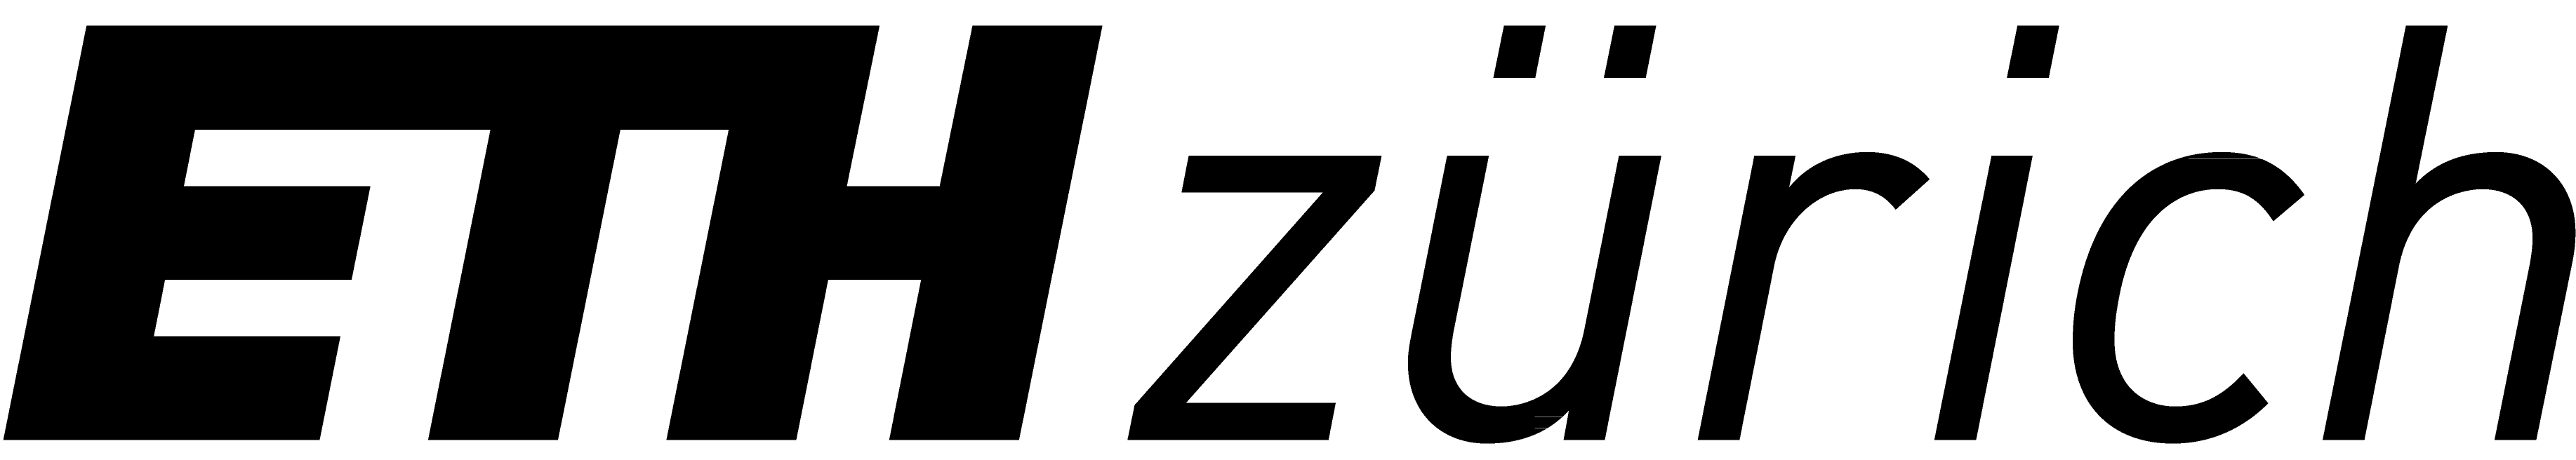
\includegraphics[height=1cm]{figures/logos/ethz.png}
% \qquad
% \includegraphics[height=1cm]{figures/logos/geg.png}
\end{center}}
%\makeatother

\begin{document}
\title{Annual report 2019:\\
{Reaktoro as the chemical reaction solver\\in Shell's reservoir simulator}}
\author{Svetlana Kyas and Allan M. M. Leal \\
{\scriptsize Institute of Geophysics, Department of Earth Sciences, ETH Z\"urich, Switzerland}}
\date{29.11.2019}

\maketitle

\section*{Summary}

The main goals of this project are:
\begin{itemize}
\item Accelerate geochemical reaction calculations (chemical equilibrium
and chemical kinetics) in reactive transport simulations using an
on-demand machine learning (ODML) algorithm.
\item Implement missing geochemical capabilities and models in Reaktoro
such as redox reactions, ion exchange, surface complexation, solid solutions. 
\item Implement native support for PHREEQC databases in Reaktoro.
\end{itemize}
During this past year (the first year of this three-year project), we
have primarily focused on advancing the first goal above (the most
challenging deliverable among the others). We summarize below the
results achieved so far, followed by the major tasks we will concentrate
next year. 
\begin{center}
\textbf{\emph{\small{}The summary below aims to be self-contained in communicating the latest achievements of this project in a concise way. However, for a deeper understanding of some parts, further reading of the subsequent sections and an attached manuscript might be required.}}{\small\par}
\par\end{center}

\subsection*{Achievements in the past year}

\subsubsection*{\emph{Further improvements in the chemical equilibrium algorithm accelerated with ODML}}

Accelerating chemical equilibrium calculations will always be mission-critical in 
the simulation of reactive transport phenomena. 
The main reason for this is the assumption of aqueous and gaseous species (as well 
as some fast-reacting minerals) to react under an instantaneous chemical equilibrium 
model. Such an approach simplifies the modeling significantly since the rates of those 
reactions are in general much faster than the rates of subsurface transport processes.

We extensively tested the on-demand machine learning algorithm
in a 1D reactive transport problem, where all chemical reaction processes
are assumed to be controlled by chemical equilibrium. 
In the simulations, we considered a mesh with 100 cells, and we executed 
10,000 time-steps. This required
1,000,000 equilibrium calculations, one per mesh cell during each time-step. The Pitzer activity model was used to represent the non-ideal
thermodynamic behavior of the aqueous solution. The choice of using the 
Pitzer model is justified  by its superior accuracy compared to others
(Davies, Debye-H\"uckel). It is also one of the most computationally
expensive aqueous activity models in the literature. The modeled chemical
system consisted of 36 species in 4 phases (an aqueous phase and three
mineral phases, namely, calcite, dolomite, and quartz). Our obtained
results are listed below:
\begin{itemize}
\item A speedup of \textbf{200}\textbf{\emph{x}} for the chemical equilibrium calculations in the reactive transport simulations.
\item The estimated upper bound for this speedup is
\textbf{400}\textbf{\emph{x}} (assuming we have a perfect, zero-cost search operation in the algorithm). This shows we can still improve the current speedup even further.
\item Only \textbf{258} chemical equilibrium states out of \textbf{1,000,000}
are fully evaluated (by triggering a Gibbs energy minimization computation (GEM));
the rest, \textbf{99.97\%}, are quickly and accurately predicted;
\item The relative error of the predictions is less than 1\% for mineral
phase volumes and less than 4\% for aqueous species concentrations for the 
chosen tolerance parameters. 
\end{itemize}

\subsubsection*{\emph{Manuscript submitted for publication}}

A manuscript entitled \emph{Accelerating Reactive Transport Modeling:
On-Demand Machine Learning Algorithm for Chemical Equilibrium Calculations
}was submitted to the journal of Transport in Porous Media on November
22nd, 2019. It presents our latest achievements on accelerated
reactive transport simulations when using ODML to speed up exclusively
chemical equilibrium calculations. A summary of this manuscript is
presented in this report. We plan to submit a follow-up manuscript
on accelerating chemical kinetics in reactive transport
simulations next year.

\subsubsection*{\emph{Chemical kinetics accelerated with ODML }}

We have already obtained preliminary results on using the ODML algorithm to speed up chemical
kinetics of mineral dissolution\slash precipitation reactions in reactive
transport simulations for a dolomitization problem in which calcite dissolves
kinetically:
\begin{itemize}
\item a speedup of \textbf{8-10}\textbf{\emph{x}} for the chemical kinetics
computations (compared to the conventional algorithm implemented in
Reaktoro); 
\item a speedup of \textbf{30}\textbf{\emph{x}} when combining accelerated
chemical kinetics of mineral dissolution with accelerated chemical
equilibrium calculations for the aqueous species.
\end{itemize}
When more than one kinetically-controlled mineral reaction is considered,
this is what we have obtained so far:
\begin{itemize}
\item a speedup of \textbf{35-102}\textbf{\emph{x}} with two kinetically-controlled
minerals and
\item a speedup of \textbf{92-124}\textbf{\emph{x}} with three kinetically-controlled
minerals. 
\end{itemize}
\textbf{Remark: }These results are a product of a few months of numerical
experimentation, and the speedups listed above can be increased with
our research plans and ideas outlined later.

\subsubsection*{\emph{Rok, a reactive transport simulator (in its early stages) using
Reaktoro and Firedrake}}

Together with a collaborator, an expert in finite element methods
and a long-time user and contributor of Firedrake (\texttt{\href{http://firedrakeproject.org}{firedrakeproject.org}}),
a Python library for solving partial differential equations, we developed
a proof of concept of a reactive transport simulator: \textbf{Rok}.
In this newly developed code, Reaktoro is used for the chemical reaction
calculations and Firedrake for the solution of the coupled governing
partial differential equations (species transport, Darcy equation,
etc.). This simulator has allowed us to perform more interesting reactive
transport simulations, considering higher-dimensions (2D) and strongly
heterogeneous porous media. We plan to use Rok not only for simulations
in general but also as a testing platform to ensure that the ODML
algorithms, we are developing, work optimally under more challenging
geochemical and geologic conditions. 

We believe this project will also be helpful to Shell, as a demonstration
on how Reaktoro can be coupled with other codes to develop
reactive transport simulators. 

\subsection*{Planned research tasks for next year}

\subsubsection*{\emph{Improving the search operations in the algorithm}}

In the on-demand learning algorithm (ODML), a new chemical equilibrium\slash kinetics
calculation is performed by first searching for previously solved
problems with similar input conditions. We currently use a nearest
neighbor search approach, in which Euclidean distances are used to
compare the new input vector with those previously computed.
The nearest neighbor problem is then used to estimate the solution
of the new problem, using exact sensitivity analysis (delivered with the
use of modern automatic differentiation strategies). 

We have observed, however, that sometimes the nearest neighbor is
not necessarily the most adequate reference point from which a prediction
is performed, which ends up causing many unnecessary training operations.
This is particularly more pronounced when the complexity of the chemical
system increases, which leads to an increased dimensionality of the
input space. Our research plan to resolve this issue is to explore
alternative search procedures. For instance, we can rank each previously
solved problem in terms of how often it was used as a reference problem
to successfully predict others. We could start our search by testing
these key problems first. We could even limit the maximum number of
stored trained problems. Only those that have been successfully
used to estimate\slash predict others and has a \emph{rate-of-use}
higher than a tolerance would be kept in a dynamic knowledge database. 

\subsubsection*{\emph{Improving the acceptance criteria in the algorithm}}

The on-demand learning algorithm can entirely bypass the iterative
computing processes of solving chemical equilibrium and kinetics problems.
The approximated solutions of these problems need, however, to be
accepted or rejected based on some given \emph{acceptance criteria}.
A rejection triggers a new training operation. This consists of an actual
solution of the problem, 
using a conventional GEM algorithm, followed by a sensitivity analysis
operation (which produces some special derivatives that 
enable quick and fast prediction of future problems
with similar input conditions). 

Currently, our acceptance criteria sometimes trigger more training
operations than it should (i.e. some predictions could have been safely
accepted, but are otherwise marked as not accurate enough). We plan
to improve the acceptance criteria in the ODML algorithm by using,
for example, \emph{measures of disequilibrium of reactions}. For example,
if the saturation index of a mineral that should be in equilibrium
is estimated to be sufficiently far from it, we then decide
that the predicted equilibrium state is not accurate enough, therefore,  it
must be exactly computed, using a GEM algorithm (followed by the 
sensitivity analysis operation). 
%
This proposed test is potentially more adequate than the one we currently
use: if predicted species chemical potentials change
by more than, say, 10\%, compared to the reference chemical potentials,
we declare the ODML prediction not accurate
enough, and new training is performed. 

\subsubsection*{\emph{Accelerate chemical equilibrium calculations when evaluating
reaction rates}}

Reaction rates of mineral dissolution\slash precipitation processes
require, in general, the saturation index of the minerals. This, in
turn, requires a chemical equilibrium calculation for the aqueous\slash gaseous
species. We plan to accelerate the evaluation of reaction rates by
speeding up these chemical equilibrium calculations, which may be
needed many times in a single kinetic time-step. 

\subsubsection*{\emph{Test the on-demand learning algorithm on more complex scenarios}}

So far, we have mainly used a 1D reactive transport example, representative
of a dolomitization process, to test the accelerated chemical equilibrium\slash kinetics
algorithms. We plan to use Rok for testing the accelerated chemical
algorithms in higher dimensions, in more complex geologic and chemical conditions.
We also intend to model a highly complex reactive transport process
resulting from the  attack of seawater into cement and concrete
systems (with collaborators from the Paul Scherrer Institute, Switzerland).
In this problem, we will consider \textasciitilde 100 aqueous species,
\textasciitilde 60 pure minerals, and \textasciitilde 10 solid solutions. 

Furthermore, we will also consider more complex cases for chemical
kinetics, including more minerals under kinetic control. 
The first results of such examples are presented in 
Appendix \ref{subsec:example-2-reactions}.

\subsubsection*{\emph{Other numerical and computational tasks}}

We also plan to:
\begin{itemize}
\item further develop Rok to enable multiphase flow and heat transfer capabilities;
\item improve support for modeling redox reactions in Reaktoro;
\item decoupling of specific surface area from the reaction definition,
so that different surface areas (for each mineral) can be set across
the reservoir if needed;
\item integrating our newly developed numerical optimization library, Optima,
into Reaktoro for more robust and faster Gibbs energy minimization
calculations;
\item compare the backward differentiation formula (BDF) schemes provided
by CVODE (the solver we currently use to solve ordinary differential
equations) with RADAU algorithms (higher-order, implicit in time,
Runge-Kutta methods) for numerical integration of the system of ODEs, to select the best solver for stiff ODE-systems describing
kinetically controlled species;
\item compare the performance of Reaktoro and PHREEQC on a set of benchmarks
provided by Shell;
\item together with collaborators from the Paul Scherrer Institute, improve
the support of thermodynamic databases in Reaktoro, including those
from PHREEQC.
\end{itemize}
\begin{center}
\textbf{\emph{Priority will be given to tasks related to extending
the modeling capabilities of Reaktoro and those that further improve
the on-demand learning algorithms for faster chemical equilibrium\slash kinetics
calculations. }}
\par\end{center}

\section{Introduction}

%---------------------------------------------------------------------------------------------------%
In reactive transport simulations, coupled chemical and physical processes are modeled to understand 
phenomena that involve the transport of chemical species (i.e. reactants) and chemical reactions. 
Examples of chemical processes are reactions between species in an aqueous fluid leading to 
precipitation of solid minerals, or their reaction with existing rock minerals causing mineral 
dissolution (see \cite{Lichtner1985, Steefel2005, Steefel2019} and references therein). Examples of 
physical processes are the advection of chemical species in a fluid that flows with a certain 
velocity, or the diffusion of those fluid species as a result of the concentration gradient across 
the medium. Because of the various processes combined into a reactive transport model, the resulting 
computer simulations are usually time-consuming.

%---------------------------------------------------------------------------------------------------%
Often, the relatively long computing time of reactive transport simulations can be largely attributed 
to the need of performing millions to billions of chemical reaction calculations, in particular, 
\emph{chemical kinetics} and\slash or \emph{equilibrium speciation calculations} performed in every 
mesh cell during every time-step of the simulation. These chemical reaction calculations are 
computationally expensive because they involve iterative algorithms to solve systems of non-linear 
algebraic and\slash or system of ordinary differential equations (ODEs) \citep{Leal2017}. As a result, 
they trigger repeated evaluations of thermodynamic properties, such as activity\slash fugacity 
coefficients (sometimes using computationally demanding models such as \citet{Pitzer1973} for aqueous 
phases and \citet{Peng1976} for gaseous/liquid phases).

%---------------------------------------------------------------------------------------------------%
Thus, speeding up reactive transport modeling by a significant factor may only be accomplished by 
first accelerating chemical reaction calculations in general. Advancing chemical equilibrium speciation 
calculations is essential when employing a \emph{partial local chemical equilibrium assumption} 
\citep{Ramshaw1980,Ramshaw1981,Ramshaw1985,Ramshaw1995,Lichtner1985,Steefel1994,Steefel1996}.
This assumes that the species that are reacting at relatively high rates (typically aqueous and gaseous 
species) are in a state of continual chemical equilibrium in each mesh cell. In contrast, the species 
reacting at slow to moderate rates (typically minerals) do so according to kinetic rate laws and, 
hence, are not in equilibrium with the rest of the system. Thus, accelerating those millions to 
billions of chemical calculations over the course of a massive numerical reactive transport simulation 
is essential when using fine-resolution meshes, large three-dimensional domains, and\slash or long 
simulation times at fine temporal resolution.

%---------------------------------------------------------------------------------------------------%
Major advances in developing fast, accurate, and robust methods for chemical equilibrium calculations, 
in particular, have been achieved over the past decades. These are either based on 
\emph{Gibbs energy minimization} (GEM) or \emph{law of mass action} (LMA) formulations 
\citep{White1958,Smith1980,Smith1982,Alberty1992b,Crerar1975,DeCapitani1987,Eriksson1989,Ghiorso1994,
Gordon1971,Gordon1994a,Gordon1996,Harvey2013,Harvie1987,Karpov1997,Karpov2001,Karpov2002,Koukkari2011a,
Kulik2013,Leal2013,Leal2014,Leal2016a,Leal2016c,Leal2017,Morel1972,Neron2012,Nordstrom1979,
Trangenstein1986,VanZeggeren1970,Vonka1995,Wolery1975,Zeleznik1960}.
%
However, even if one could devise a hypothetical algorithm that would always converge in a single 
iteration, instead of the typical few to dozens of iterations, the computational cost of chemical 
equilibrium calculations could still be dominant in a reactive transport simulation. This is the case, 
as during this single iteration expensive thermodynamic models would still have to be evaluated and 
matrix equations have to be solved (using a Newton-based GEM or LMA algorithm). In view of this, 
a substantial acceleration of these calculations can be achieved if those costly operations
can be bypassed whenever possible. 

Similarly, advanced methods for solving a system of differential equations has been 
developed during a couple of last decades \cite{Ascher1998,HairerNorsettWanner1993,HairerWanner1996}. 
Due to rapid variations in some of the species' reaction rates, the behavior of kinetically-controlled 
species are often represented by the stiff system of ODEs, which adds additional difficulty. 
However, we aim to apply such an approach that sidesteps costly numerical integration of the system 
that governs the evolution of kinetics species within considered transport step.

\begin{figure}[!t]
	\centering
	\subfloat[]{
	\includegraphics[height=6cm]{figures/intro/similar-equilibirum}
	\label{fig:similar-equilibrium}}
	\quad
	\subfloat[]{
	\includegraphics[height=6cm]{figures/intro/similar-kinetics}
	\label{fig:similar-kinetics}}
	\caption{Example of similar chemical speciations encountered in chemical equilibrium and kinetics.}
	\label{fig:similar-kinetics-equilibrium}
\end{figure}

%---------------------------------------------------------------------------------------------------%
During a single time-step of a reactive transport simulation, chemical kinetics and equilibrium
calculations are needed in all mesh cells. Often, many of these calculations are similar to previously 
performed ones, either within the same time-step and\slash or mesh cell or at different points in 
space and\slash or time (see Figure \ref{fig:similar-kinetics-equilibrium}). We assume two chemical 
equilibrium problems to be similar when their input conditions are sufficiently close (i.e., similar 
temperature, pressure, amounts of chemical elements, and the electric charge of each phase, containing 
electrically charged species \citep{Smith1982}). At the same time, these chemical equilibrium 
calculations are hardly identical so that we cannot simply assume a previously computed chemical 
speciation as the exact result of the new calculation. Interpolating is also not an appropriate
approach, as it can violate the \emph{mass conservation} of elements (i.e., there is a deviation 
between the input element amounts and the amounts of elements calculated from the interpolated species 
amounts). 

%---------------------------------------------------------------------------------------------------%
The main principle of the \emph{ODML algorithm} suggested here is precisely to \emph{avoid} as much as 
possible full and expensive chemical speciation calculations during the reactive transport simulation. 
That is why it is often referred to as \emph{smart chemical equilibrium algorithm}. By using 
\emph{sensitivity derivatives} of previously computed chemical equilibrium states, we can quickly 
and accurately estimate the new equilibrium state (chemical speciation) under similar input conditions
(see Figure \ref{fig:similar-equilibrium}). These derivatives provide an insight into how sensitive
the computed species amounts at a certain equilibrium state are with respect to infinitesimally small 
changes in temperature, pressure, and amounts of chemical elements. Thus, multiplying these sensitivity 
derivatives by the respective differences in input conditions (e.g., differences in temperature
or the amount of a particular element), we can predict the variation in the output. For example, we 
can estimate how much the species amounts would change by increasing temperature by 1~°C, by adding 
1~mmol of HCl into the system (which is equivalent to adding 1~mmol of elements H and Cl), or by 
combining these with other input changes. We remark that the use of sensitivity derivatives to estimate 
the solution of an equilibrium problem is inherently \emph{mass conservative} since they are being 
computed along with the derivation of chemical equilibrium equations (with equations of element mass 
conservation included).

%---------------------------------------------------------------------------------------------------%
For kinetically controlled species, one can find similarities in their initial 
states at each transport step. Figure \ref{fig:similar-kinetics} illustrates possible perturbations 
of fluid/rock compositions in mesh cells discretising a two-dimensional reservoir. \emph{Smart chemical 
kinetics algorithm} will perform numerical integration of the system of kinetic species only for 
some uniquely distinguishable initial states \emph{(marked with empty circles in Figure 
\ref{fig:similar-kinetics})}. Simultaneously, we also recover additional information about their 
sensitivities with respect to infinitesimal changes in the initial condition. In the rest of the 
subsequently encountered cells, we attempt to make \emph{smart prediction} of the possible kinetic 
speciation at the end of the transport step, exploiting information collected in the previous 
mesh-cells.

\subsubsection*{Related Work}

Increasing the speed of chemical speciation calculations, whether it is equilibrium and\slash or 
kinetics, is an active research topic. The majority of the existing methodologies are based on the use 
of \emph{surrogate models} and\slash or \emph{statistically-based machine learning} schemes, which use 
a computationally cheaper model (e.g., linearization, parameterization, convolutional neural network) 
to approximate a complex nonlinear behavior.

%---------------------------------------------------------------------------------------------------%
In combustion chemistry, the pioneering work of \citet{Pope1997} in accelerating \emph{chemical 
kinetics calculations} considered approximations of chemical kinetics paths using multiple linear 
regressions, employing \emph{unstructured adaptive} \emph{storage/extraction techniques} along 
the simulation process. This approach is referred to in the literature as the \emph{in-situ adaptive 
tabulation} (ISAT) algorithm. The ISAT approximation idea was later extended to \emph{nonlinear
model predictive control} (NMPC) in \citep{HedengrenEdgar2008}. ISAT can be regarded as an alternative 
to artificial neural networks, as it does not require any preliminary training to simulate the 
behavior of the model. Instead, it rearranges the model by the training on new data \emph{on the 
fly}, as simulations proceed. The ISAT algorithm scales quadratically with increased dimension, 
approximates functions with discontinuities, and provides explicit bounds on approximation errors. 
Recent improvements of the ISAT algorithm and\slash or its demonstration for the simulation of 
unsteady, compressible, reactive flows can be found in 
\cite{Singer2004,Singer2006,Lu2007,Pope2009,Lu2009}.
%
A series of parallel chemistry acceleration algorithms using different distribution strategies for
simulation of unsteady, compressible, reactive flows, based on the ISAT technique, was implemented in 
the software \texttt{\href{https://tcg.mae.cornell.edu/x2f\_mpi/}{${\rm x2f_mpi}$}} \cite{x2fmpi2006} 
and studied for the numerical simulations of a two-dimensional gaseous detonation wave propagation 
process in \citet{Dong2007,Dong2009,WuDongLi2018}. 

%---------------------------------------------------------------------------------------------------%
In addition to the ISAT approach, several alternative storage-based approaches have been suggested in 
the past for accelerating chemical kinetics calculations, including polynomial fits \citet{Turanyi1994}, 
artificial neural networks (see, e.g., \citet{ChristoMasriNebot1996,Blascoetall1998}), and piece-wise 
reusable implementation of solution mapping (PRISM) by \citet{TonseMoriartyBrownFrenklach2013}. The 
common property of these approaches is the a priori creation of the approximation model (whether it 
is a skeleton model or a neural network), which usually requires extra effort to then evaluate a 
simplified model that accelerates subsequent calculations. The PRISM method is similar to the in-situ 
approach, except that the stored data entries are not output values and corresponding sensitivity 
derivatives, but rather the set of polynomials, covering a region of chemical composition space. 
The observed acceleration for these methods is about a factor of 10-60.

%---------------------------------------------------------------------------------------------------%
The work of \citet{Jatnieks2016}, on the use of a surrogate model for fast speciation calculations, 
is another initiative to accelerate chemical equilibrium calculations during reactive transport 
modeling. The construction of this surrogate model required a training stage in advance of the 
simulation of interest, during which many random input conditions are used in PHREEQC 
\citep{Parkhurst2013}, and the resultant outputs collected for statistics-based 
learning. During their numerical experiment,~32~different statistical and machine learning methods
were tried to identify the potentially best one. For a specific reactive transport modeling problem, 
\citet{Jatnieks2016} collected all possible input-output combinations in speciation calculations, and 
from these, 7880 input-output samples, representing 80\% of the total known input-output relationships, 
were used for training the statistical model. The various constructed surrogate models were subsequently 
used in the reactive transport simulation. Because these surrogate models relied on statistical methods, 
mass conservation was often not accurate during their machine learning computations (i.e., the amounts 
of chemical elements in the estimated-output species amounts did not correspond accurately to the 
values given in the input). 

The work \cite{Laloy2019} presents a comparison of several approaches 
(Gaussian processes (GP), polynomial chaos expansion (PCE) and deep neural networks (DNNs)), which are 
used to emulate CPU-intensive reactive transport models. However, considered methods are subjected 
to uncertainties propagation and, as a result, deteriorating accuracy. For relatively simple problems 
DNNs performed the best (even having relatively small training sets), providing the most accurate 
representation of results. However, the DNN approach leads to the worst solution of the considered 
synthetic inverse problem due to the small but rather complicated deterministic noise that affects 
the DNN-based predictions. Also, for more complicated problems DNN produces quite disperse outputs, 
which only confirms the difficulty of finding emulator able to replace the entire reactive transport 
process with all its complex behaviours and possible outcomes. The approach proposed in our work 
focuses only on speeding up the chemical part of the entire simulation, which narrows down the number 
of physical effects influencing the input space and, as results, allows finding more similarities 
triggering more smart predictions.
%
Moreover, unlike the ``black-box'' representation of the complex original model used by methods in 
\cite{Laloy2019}, our approach ``remembers'' the most crucial properties of the chemical system under 
consideration (such as mass balance equation, sensitivity derivatives, ect.), allowing to maintain 
the requested accuracy of simulations' results.

We acknowledge yet another approach that provides the means for automation 
of the speciation for thousands of similar scenarios called \emph{smart-Kd} 
(\citet{Stockmann2017}), which has a high potential to increase confidence 
and reduce conservatism in long-time safety assessment studies or other 
contaminant migration scenarios.
%
It is based on a mechanistic understanding of basic sorption processes such 
as surface complexation, ion exchange, surface precipitation and incorporation. 
It uses \emph{component additivity} and a \emph{generalized composite} approaches
to compute distribution coefficients (Kd-values), which are then used 
to efficiently reproduce a broad variety of (geo)chemical conditions.
%
The component additivity approach is an attempt to predict adsorption on 
a complex mineral assemblage, using the results of a surface characterization 
of the assemblage and collected data for adsorption by pure, reference minerals 
or organic phases. 
In the generalized composite approach, the adsorptive reactivity of the surface 
is described by surface complexation equilibria written with ``generic'' surface 
functional groups (with the stoichiometry and formation constants for each 
equilibria determined by fitting experimental data).
%
The smart-Kd uses high-quality thermodynamic databases to compute
aqueous speciation and the assemblage of minerals being in equilibrium
with this solution, as well as all surface species. 
%
This opens a path to more complex applications with respect to support
large-scales models by multidimensional look-up tables of Kd-values,
as well as for comprehensive uncertainty and sensitivity analysis.

\subsubsection*{Advantages of the ODML algorithm}

%---------------------------------------------------------------------------------------------------%
The \emph{on-demand learning approach} developed here exhibits several advantages over conventional 
statistics- or neural network-based machine learning methods. Firstly, the use of \emph{sensitivity 
derivatives} of the calculated equilibrium states results in a method that better reflects the behavior 
of chemical systems and how they react to subsequent changes in input equilibrium conditions. Secondly, 
the use of these sensitivity derivatives permits predicting new equilibrium states \emph{with accuracy and confidence} using relatively little amount of data. Thirdly, the proposed method requires \emph{no a priori statistical 
training} before it can be applied in a reactive transport simulation. Its on-demand machine learning 
characteristics enable spontaneous learning of only what is needed to be calculated anew during 
a reactive transport simulation to keep new predictions accurate enough. Note that, when using 
a conventional chemical equilibrium calculation approach, these computations are needed anyway. 

%---------------------------------------------------------------------------------------------------%
Furthermore, the on-demand learning strategy is not only simpler from an end-user point 
of view (as no a priori training stage needs to be performed), but also likely faster. It will, 
in general, require saving far fewer input conditions and computed chemical speciations than any 
statistical approach, which can only get the more accurate the more it trains in advance, and where 
the amount of useful training calculations is unknown. This lack of knowledge typically leads to 
the calculation of many more chemical reaction results than what may ever be needed during the actual 
simulation, with a risk that actually required calculations may not have been part of the a priori 
training set at all. This is akin to going to school to learn all sorts of things, most of which are 
never needed later on for a specific job at hand. 

%---------------------------------------------------------------------------------------------------%
Finally, the on-demand accelerated chemical reaction algorithms (equilibrium\slash kinetics) produce chemical states that \emph{always 
satisfy conservation conditions} for chemical elements and electric charge, as these constraints are 
incorporated into the calculation of the sensitivity derivatives (see \citet{Leal2017}). This, in 
particular, distinguishes the discussed method from the statistics-based machine learning methods, 
which can lose accuracy or fail in this respect.

Some similarities may inevitably exist between the \emph{on-demand machine learning} (ODML)
algorithm and other existing strategies for speeding up chemical equilibrium 
and\slash or chemical kinetics calculations. Existing techniques, for example, that 
rely on interpolation, may also require search operations and decision making whether 
to accept or not the interpolated estimate. However, the major current (and also future) 
differences are that ODML
%
\begin{enumerate}[wide, labelwidth=!, labelindent=0pt]
\item[\emph{(i)}] aims to be a more \textbf{general-purpose acceleration algorithm} that could also 
be applied for other types of expensive and repeated computations (e.g. evaluations of fluid 
thermo-physical properties) instead of being applied exclusively to chemical equilibrium and\slash or 
chemical kinetics problems;
%
\item[\emph{(ii)}] can use \textbf{higher-order sensitivity derivatives} for improved predictive 
accuracy that reduces the number of on-demand training operations, and provide superior error 
analysis (detailed in a future communication);
%
\item[\emph{(iii)}] provides the capability for \textbf{more flexible error controls} that may 
consider chemical, physical, and\slash or engineering insights on the acceptance decision, instead 
of relying on statistics or geometric considerations (e.g., using hyper-ellipsoids confidence regions); 
and, finally,
%
\item[\emph{(iv)}] uses \textbf{alternative search operations} that do not rely exclusively on 
the nearest neighbor search, which is prone to fail for high-dimensional input spaces (commonly-known 
in the statistical and machine learning literature as the \emph{curse of dimensionality}).
\end{enumerate}
%
%---------------------------------------------------------------------------------------------------%
A dedicated C++ library project for ODML is envisioned, in which the exact higher-order sensitivity
derivatives mentioned previously are calculated using 
\texttt{\href{http://autodiff.github.io}{autodiff}} (\citealt{autodiff}), a modern and fast C++ 
library for higher-order automatic differentiation computations, whose on-going development is 
specifically carried out towards achieving the planned algorithm's goals.

%---------------------------------------------------------------------------------------------------%
\subsubsection*{Organization}

This report is organized as follows:
\begin{enumerate}[wide, labelwidth=!, labelindent=0pt]
\item [{\bf Section~\ref{sec:Definitions-and-Notation}}] introduces definitions and the notation 
needed to describe the algorithm.
\item [{\bf Section~\ref{sec:Method}}] formulates the ODML algorithm and its application to accelerate chemical equilibrium and kinetics 
calculations.
\item [{\bf Section~\ref{sec:Results}}] demonstrates the performance and accuracy of a reactive 
transport simulation using the on-demand learning accelerated chemical equilibrium and kinetics algorithms. 
%
% Let's keep this short.
% It consists of three parts 
% with results corresponding to three major stages of development of algorithms. The first tests
% of the algorithm were focused on studying its performance in the reactive transport model with all 
% the species controlled
% by equilibrium and with Pitzer activity model used (see Subsection \ref{subsec:part-1}). 
% %
% Subsection \ref{subsec:part-2} is dedicated to describing the performance of the smart approach on 
% the chemical system with kinetically controlled species. 
%
% Finally, Subsection \ref{subsec:part-3} highlights results of reactive transport simulations 
% obtained after coupling \texttt{Reaktoro} with \texttt{Firedrake}, an automated system for the 
% solution of partial differential equations (PDEs) using the finite element method (FEM) 
% \cite{Rathgeber2016}.

\item [{\bf Section~\ref{sec:Discussion-and-Conclusions}}] concludes the report and discusses the work performed so far and a road-map for further research efforts.
\end{enumerate}

%---------------------------------------------------------------------------------------------------%
\section{Definitions and Notation\label{sec:Definitions-and-Notation}}

Considered throughout this report, a \emph{chemical system} is a collection of \emph{chemical species} 
composed of one or more \emph{elements} and distributed among one or more \emph{phases}. The species 
can be substances such as aqueous ions (e.g., Na$^{+}$(aq), Cl$^{-}$(aq), HCO$_{3}^{-}$(aq)), neutral 
aqueous species (e.g., SiO2(aq), CO$_{2}$(aq), H$_{2}$O(l)), gases (e.g., CO$_{2}$(g), CH$_{4}$(g), 
N$_{2}$(g)), pure condensed phases (e.g., CaCO$_{3}$(s, calcite), SiO$_{2}$(s, quartz), 
Al$_{2}$Si$_{2}$O$_{5}$(OH)$_{4}$(s, kaolinite)), etc. Each phase (e.g., aqueous, gaseous, liquid, 
solid solutions, a pure mineral, plasma, etc.), having homogeneous properties within its boundaries 
is composed of one or more different chemical species (components, end members). Multi-component 
phases are also called \emph{solutions}, where components are mixed within the same structure.  
The elements (independent components) are \emph{chemical elements} (e.g., H, O, C, Na, Cl, Ca, Si) 
and \emph{electrical charge} (Z), but can also be linear combinations of these, commonly known as 
\emph{primary species} (e.g., H$^{+}$(aq), H$_{2}$O(l), CO$_{2}$(aq)).

A chemical system can exist at infinitely many \emph{chemical states}. A chemical state is defined 
here as the triplet $(T, P, n)$, where $T$ is temperature, $P$ is pressure,  
$n=(n_{1},\ldots,n_{\mathrm{N}})$ is the vector of species amounts 
(speciation), with $n_{i}$ denoting the amount of the $i$th species (in moles) and N the number of 
species. The vector of element amounts is defined by 
$b=(b_{1},\ldots,b_{\mathrm{E}})$ is the vector of element 
amounts with $b_{j}$ being the amount of the $j$th element (in moles) and ${\rm E}$ the number of 
elements. In general, $b$ is related to $n$ via the following mass conservation equation:
%
\begin{equation}
An=b,
\label{eq:mass-balance}
\end{equation}
%
where $A$ is the \emph{formula matrix} of the chemical system \citep{Smith1982} (whose dimensions 
are $\mathrm{E}\times\mathrm{N}$), with $A_{ji}$ denoting the coefficient of the $j$th element in 
the $i$th species.

In order to model a chemical system with a mixing of equilibrium- and kinetically-controlled 
reactions, we classify the species in two groups: \emph{equilibrium species} and \emph{kinetic species}. Their corresponding amounts are represented as
$n_{e} \in \mathbb{R}^{{\rm N}_e}$ and $n_{k} \in \mathbb{R}^{{\rm N}_k}$, where 
${\rm N} = {\rm N}_e + {\rm N}_k$, and corresponding elements compositions 
$b_{e}, b_{k} \in \mathbb{R}^{\rm E}$. 
Then, the vector of species amounts (including both equilibrium and 
kinetic species) is 
\[
n=\begin{bmatrix}n_{e}\\n_{k}\end{bmatrix} 
\]
with the formula matrix $A=\begin{bmatrix}A_{e}\;A_{k}\end{bmatrix}$ composed of 
the formula matrices of the equilibrium and kinetic species $A_{e}$ and $A_{k}$, respectively. 

%---------------------------------------------------------------------------------------------------%
\section{Method\label{sec:Method}}

%---------------------------------------------------------------------------------------------------%
Evolving the chemical state of a system subject to equilibrium- 
and kinetically-controlled reactions requires the solution of the following
system of ordinary differential equations:
%
\begin{alignat}{2}
\frac{\mathrm{d}b_{e}}{\mathrm{d}t} & =A_{e}(q_{e}+\nu_{e}^{{\rm T}}r) & \qquad & t>0\label{eq:kinetics-1}\\
\frac{\mathrm{d}n_{k}}{\mathrm{d}t} & =\nu_{k}^{{\rm T}}r+q_{k} &  & t>0\nonumber \\
b_{e} & =An_{e}^{\circ} &  & t=0\nonumber \\
n_{k} & =n_{k}^{\circ} &  & t=0\nonumber 
\end{alignat}
%
%---------------------------------------------------------------------------------------------------%
where $r=(r_1,\ldots, r_{\mathrm{M}_k})$ is the vector of \emph{rates} of the kinetically-controlled reactions, $q_{k}$ denote
the vector of  \emph{inflow/outflow rates of the kinetic species}, $n_{k}^{\circ}$ is
vector of the \emph{initial amounts of the kinetic species}, and $\nu_{k} \in \mathds{R}^{{\rm M}_k \times 
{\rm N}}$ and $\nu_{e} \in \mathds{R}^{{\rm M}_e \times {\rm N}}$ are the matrices formed from 
the columns of the stoichiometric matrix $\nu=\begin{bmatrix}\nu_{e}\,\nu_{k}\end{bmatrix}$ with
${\rm M}_k$ and ${\rm M}_e$ corresponding to the number of kinetic and equilibrium reactions, 
respectively.
%
For a more detailed derivation of these equations, we refer to \citet{Leal2015,Leal2017}.

The previous equations solve for the amounts of each element in the equilibrium
partition ($b_e$) and the amounts of each species in the kinetic partition ($n_k$).
To calculate the amounts of each species in the equilibrium partition ($n_e$), 
we perform a chemical equilibrium calculation, which we denote abstractly as
%
\begin{equation}
n_{e}=\varphi(T, P, b_{e}),
\label{eq:equilibrium-func}
\end{equation}
%
where $\varphi$ is
a chemical equilibrium function that encapsulates the 
specific algorithmic steps to solve the fundamental Gibbs energy minimization 
problem
%
\[
\varphi(T, P, b_{e}) \coloneqq \mathop{\mathrm{argmin}}_{n_{e}} G_{e} = n_{e}^{\rm T} \mu_{e}
\quad\mbox{subject to}\quad
\left\{ \begin{aligned}A_{e}n_{e} & =b_{e}\\
n_{e} & \geq0
\end{aligned}
\right..
\label{eq:gem-problem}
\]
%
The \emph{chemical potential} of the $i$th species $\mu_{e, i}=\mu_{e, i}(T,P,n)$ is defined as:
%
\begin{equation}
\mu_{e, i}=\mu_{e, i}^{\circ}+RT\ln a_{e, i},
\end{equation}
%
with $R$ denoting the universal gas constant, $\mu_{e, i}^{\circ}=\mu_{e, i}^{\circ}(T,P)$ the 
\emph{standard chemical potential} of the $i$th species, and $a_{e, i}=a_{e, i}(T, P, n)$ the 
\emph{activity} of the $i$th species. Methods for solving chemical equilibrium problem using 
either Gibbs energy minimization (GEM) or the law of mass action (LMA) methods are addressed in 
more details in \citet{Leal2016a,Leal2016c,Leal2017}.

Thus, the evolution of the chemical state of a system undergoing a 
mixed equilibrium and kinetic process is governed by the following 
differential-algebraic equations
%
\begin{alignat}{2}
\frac{\mathrm{d}b_{e}}{\mathrm{d}t} & =A_{e}(q_{e}+\nu_{e}^{{\rm T}}r) & \qquad & t>0\label{eq:kinetics-full-1}\\
\frac{\mathrm{d}n_{k}}{\mathrm{d}t} & =\nu_{k}^{{\rm T}}r+q_{k} &  & t>0\nonumber \\
n_{e} & =\varphi(T,P,b_{e}) &  & t>0\nonumber\\
b_{e} & =An_{e}^{\circ} &  & t=0\nonumber \\
n_{k} & =n_{k}^{\circ} &  & t=0\nonumber \\
n_{e} & =n_{e}^{\circ} &  & t=0\nonumber
\end{alignat}
%
where $n^\circ = [n_{e}^{\circ},n_{k}^{\circ}]^{\rm T}$ is a given initial condition
and $T$ and $P$ are also given and constant.

\subsection{First-Order Taylor Approximation\label{subsec:First-order-Taylor-approximation}}
%---------------------------------------------------------------------------------------------------%
Let the process of solving the mathematical problem in Eq.\eqref{eq:kinetics-full-1} be represented in the following functional notation:
%
\begin{equation}
    y = f(x),\label{eq:function}\\ 
\end{equation}
%
where $f$ is the function that performs the necessary steps towards a solution; $x$ is the \emph{input vector}, comprising of temperature ($T$), pressure ($P$), 
the initial amount of each species in the chemical system (vector $n^\circ$), 
and the time interval that we let the chemical system to react ($\Delta t$); $y$ is the  \emph{output vector} containing the final amount of each species in the chemical system (vector $n$) after
they were allowed to react for the given time interval. In addition to this, we also include into $y$ the vector of chemical potentials of the species, $\mu$, 
and the vector of reaction rates, $r$. In other words, the output vector not only contains the information on the final
speciation of the chemical system, but also on the key thermochemical 
properties at that final state. Mathematically, it is defined as
%
\begin{equation}
x=\begin{bmatrix}T\\
P\\
n^{\circ}\\
\Delta t
\end{bmatrix}\qquad\text{and}\qquad y=\begin{bmatrix}n\\
\mu\\
y
\end{bmatrix}.\label{eq:x-and-y-defs}
\end{equation}
%---------------------------------------------------------------------------------------------------%
%
Assume that $f$ in Eq.\eqref{eq:function} has been evaluated previously with input conditions 
$x^\star$, and a new evaluation needs to be performed with $x$ instead. Rather than computing $y$, 
using the computationally expensive function $f$, we first try estimating it with a 
\emph{first-order Taylor approximation}:
%
\begin{equation}
\bar{y} = 
x^{\star} + \frac{\partial f}{\partial x}^{\star}(x-x^{\star}),
\label{eq:smart-estimate}
\end{equation}
%
where $\bar{y}$ denotes the estimate of exact $y$, 
$(\partial f/\partial x)^{\star}$ is the Jacobian matrix of $f$ evaluated
at the reference input point $x^\star$. We call it
the \emph{sensitivity matrix} of the system at $x^\star$ because it tells us how sensitive, 
for example, the final computed chemical state is with respect to temperature,
pressure, the initial speciation of the system, and the time interval we let it react for.
Thus, we can use these derivatives to 
estimate how the species amounts in the final state would change when
small perturbations are applied to temperature, pressure, and\slash or 
initial species amounts. This can thus be used to quickly and accurately 
predict new chemical states in the vicinity of some previously and
fully calculated ones.
\textbf{Note:} Computing this sensitivity matrix efficiently and accurately 
is far from trivial, and we are able to accomplish this via the use 
of automatic differentiation. 

\subsection{Nearest Neighbor Search\label{subsec:Nearest-Neighbor-Search}}

Let $\mathcal{I} = \{x^i\}_{i=1}^{{\rm I}}$ represent the set
of input vectors $x^i$ for which $f$ has been evaluated (i.e. input conditions for the 
chemical kinetics-equilibrium problem that have been fully solved so far).
%
%---------------------------------------------------------------------------------------------------%
Furthermore, let 
%
\begin{equation}
d^{i}=||x-x^{i}||\qquad(i=1,\ldots,\mathrm{I})
\end{equation}
%
denote the Euclidean distances from a stored input vector $x^i$ to the new input vector $x$.

For the first-order Taylor expansion presented in Eq.~(\ref{eq:smart-estimate}), a potentially 
suitable candidate for $x^{\star}$ is the \emph{nearest neighbor} (NN) of $x$ among all inputs 
in $\mathcal{I}$ (i.e. the saved input $x^i$ with the shortest Euclidean distance to $x$).

\textbf{Note:} Other norms can be used to define the distance measure above and other search 
operations can be equally considered (not necessarily based on the nearest neighbor, which can be 
prone to the curse of dimensionality as the number of input parameters increases). We are 
currently investigating alternative search schemes and have already identified some with more 
promising results. However, 
for the specific reactive transport modeling problem we consider in this proof-of-concept work 
(described in Section~\ref{sec:Results}), we obtain satisfactory overall performance results with 
the nearest neighbor search scheme described above.

Plenty of algorithms have been reported in the literature to conduct a fast multi-dimensional NN 
search. The use of \emph{kd-tree data structures} to store the inputs, for example, may permit us to
obtain an algorithm complexity $\log_{2}(\mathrm{K})$, where $\mathrm{K}$ is the number of entries 
in the set. This implies that in a set with 1024~entries, only about 10 distance comparisons are 
performed. This contrasts with a linear search algorithm, with complexity $O(\mathrm{K})$,
which would instead require 1024 corresponding evaluations and comparisons.

%---------------------------------------------------------------------------------------------------%
The above algorithms, however, may behave very differently, depending on the number and dimension 
of the input vectors collected. Tree data structures have a more sparse memory pattern than 
contiguous memory data structures, such as arrays\slash vectors. The portions of the data for the 
latter can be cached by the CPU, enabling processing them at much faster rates. This implies that 
for sufficiently small data-sets (e.g, with dozens to perhaps a few hundred entries), tree-based 
search algorithms could be sub-optimal. Under these circumstances, a linear search algorithm, 
conjugated with contiguous memory data structures, can be more efficient.

%---------------------------------------------------------------------------------------------------%
In the first version of the algorithm implementation, we have relied solely on a linear search
algorithm, which worked well in the acceleration of the reactive transport problem (assuming all the 
species are controlled by equilibrium) shown in Section~\ref{sec:Results}. Complementing
the computer implementation of the smart chemical equilibrium algorithm
with kd-tree/locality-sensitive hashing search algorithms is ongoing work.

\begin{comment}
%---------------------------------------------------------------------------------------------------%
Assume that a chemical equilibrium calculation has been performed previously with input conditions
$(T^{\star},P^{\star},b^{\star}) = (T,P,b)^\star$, and a new one needs to be performed with 
$(T,P,b)$ instead. 
%
Rather than computing $n_e=\varphi(T,P,b_e)$, using the computationally expensive equilibrium 
function $\varphi$ (cf. \ref{eq:equilibrium-func}), we first try estimating $\bar{n}_e$ with a 
\emph{first-order Taylor approximation}:
%
\begin{equation}
\bar{n} = 
n^{\star}+\frac{\partial\varphi}{\partial T}^{\star}(T-T^{\star})
+\frac{\partial\varphi}{\partial P}^{\star}(P-P^{\star})
+\frac{\partial\varphi}{\partial b}^{\star}(b-b^{\star}),
\label{eq:smart-estimate}
\end{equation}
%
where $(\partial\varphi/\partial T)^{\star}$, $(\partial\varphi/\partial P)^{\star}$, and 
$(\partial\varphi/\partial b)^{\star}$ are \emph{sensitivity derivatives} of the reference chemical 
equilibrium state, which can be equivalently written as $(\partial n/\partial T)^{\star}$, 
$(\partial n/\partial P)^{\star}$, and $(\partial n/\partial b)^{\star}$, respectively. If computed 
together with the full speciation vector $n$, these sensitivity derivatives will allow us to estimate 
how the species amounts in an equilibrium state change when small perturbations are applied to 
temperature, pressure, and\slash or amounts of elements, and, therefore, quickly and accurately 
estimate entirely new states in the vicinity of some previous and fully calculated chemical 
equilibrium state.

%---------------------------------------------------------------------------------------------------%
In case of kinetically controlled species, the similar approach can be applied. We use 
the sensitivities of species $n_k$ with respect to the initial condition $n_k^\circ$ defined as
%
\[
S(t) := \frac{\partial n_k}{\partial n_k^\circ} (t). 
\label{eq:sensitivities}
\]
%
%---------------------------------------------------------------------------------------------------%
Let 
$S^\star = \Big(\tfrac{\partial n_k}{\partial n_k^\circ}\Big)^\star$ be stored along with $n^\star_k$ 
(result of numerical integration of the system defined by Eq.~\eqref{eq:kinetics}) and the initial 
state $\big(n^\circ_k\big)^\star$. Then, instead of evaluating new chemical state with the initial 
condition $n^\circ_k$, the kinetic species can be approximated as follows:
%
\begin{equation}
\bar{n}_k 
= n^\star_k + \delta n_k
= n^\star_k + S^\star \, \delta n^\circ_k
= n^\star_k + \Big(\frac{\partial n_k}{\partial n_k^\circ} \Big)^\star \, 
\big(n^\circ_k - (n^\circ_k)^\star \big).
\label{eq:smart-estimate-kinetics}
\end{equation}
%
If $\bar{n}_k$ is accurate enough, the computationally costly numerical integration of the system 
\eqref{eq:kinetics} is replaced by matrix-vector multiplication formula 
\eqref{eq:smart-estimate-kinetics}. Here, sensitivities are defined by the matrix 
$S \in \mathbb{R}^{{\rm N}_k \times {\rm N}_k}$ that satisfies the following system of ODEs
% 
\begin{align*}
\frac{\partial S}{\partial t} & = J_r (n_k) \, S & t>0,\\
             S & = I            & t=0,
\end{align*}
%
where ${J}_{r}$ is a Jacobian of $r(n_k)$, and ${I} \in \mathbb{R}^{N \times N}$ is the identity 
matrix.

%---------------------------------------------------------------------------------------------------%
\subsection{Nearest Neighbor Search\label{subsec:Nearest-Neighbor-Search}}

Let 
%
\begin{equation}
\mathcal{I}_e =\left\{ (T,P,b_e)^{\,i}\right\}_{i=1}^{{\rm I}} 
\qquad \mbox{and} \qquad 
\mathcal{I}_k =\left\{ (n^{\circ}_k)^{\,j} \right\}_{j=1}^{{\rm J}}
\end{equation}
%
represent the sets of input conditions for the chemical equilibrium and kinetics problems, 
respectively, that have been fully solved (i.e., using the chemical equilibrium function $\varphi$ 
or system of ODEs \eqref{eq:kinetics}).
%
\sveta{
%---------------------------------------------------------------------------------------------------%
Furthermore, let 
%
\begin{equation}
d^{i}_e = \left[
\left(T-T^{i}\right)^{2} 
+\left(P-P^{i}\right)^{2}
+\sum_{l=1}^{{\rm E}}\left(b_{l}-b_{l}^{i}\right)^{2}\right]^{\frac{1}{2}} 
\qquad \mbox{and} \qquad 
d^{j}_k = \left[ \sum_{m=1}^{{\rm N_k}} 
n^\circ_{k, m} - \left((n^\circ_{k, m})^{\,j}\right)^2 \right]^{\frac{1}{2}} 
\end{equation}
%
denote, respectively, the Euclidean distances from $(T, P, b_e)^i$ to $(T,P,b_e)$ and from 
$(n^\circ_{k})^{\,j}$ to $n^\circ_{k}$. In $d^{i}_e$, the input condition of the $i$th fully 
solved problem and the given input condition for the new equilibrium calculation are compared, 
whereas $d^{j}_k$ measures the distance between the initial condition of $j$th fully integrated 
problem and the initial condition of new one.
}

%---------------------------------------------------------------------------------------------------%
\textbf{Note:} Other norms can be used to define the distance measure above and other search 
operations can be equally considered (not necessarily based on the nearest neighbor, which can be 
prone to the curse of dimensionality as the number of considered elements E increases). We are 
currently investigating alternative search schemes and have already identified some with more 
promising results. These findings will be the subject of a subsequent investigation steps. However, 
for the specific reactive transport modeling problem we consider in this proof-of-concept work 
(described in Section~\ref{sec:Results}), we obtain satisfactory overall performance results with 
the nearest neighbor search scheme described before.

%---------------------------------------------------------------------------------------------------%
For the first-order Taylor expansion presented in Eq.~(\ref{eq:smart-estimate}) and 
Eq.~(\ref{eq:smart-estimate-kinetics}), a potentially suitable candidate for $(T,P,b_e)^{\star}$ and 
$(n^\circ_k)^\star$ is the \emph{nearest neighbor} (NN) of $(T,P,b_e)$ or $n^\circ_k$ among all inputs 
in $\mathcal{I}_e$ or $\mathcal{I}_k$ (i.e., saved input with the shortest Euclidean distance to 
$(T,P,b_e)$ or $n^\circ_k$). Note that other norms and strategies can be used to define the most 
optimal reference element for the prediction.

Plenty of algorithms have been reported in the literature to conduct a fast multi-dimensional NN 
search. The use of \emph{kd-tree data structures} to store the inputs, for example, may permit us to
obtain an algorithm complexity $\log_{2}(\mathrm{K})$, where $\mathrm{K}$ is the number of entries 
in the set. This implies that in a set with 1024~entries, only about 10 distance comparisons are 
performed. This contrasts with a linear search algorithm, with complexity $O(\mathrm{K})$,
which would instead require 1024 corresponding evaluations and comparisons.

%---------------------------------------------------------------------------------------------------%
The above algorithms, however, may behave very differently, depending on the number and dimension 
of the input vectors collected. Tree data structures have a more sparse memory pattern than 
contiguous memory data structures, such as arrays\slash vectors. The portions of the data for the 
latter can be cached by the CPU, enabling processing them at much faster rates. This implies that 
for sufficiently small data-sets (e.g, with dozens to perhaps a few hundred entries), tree-based 
search algorithms could be sub-optimal. Under these circumstances, a linear search algorithm, 
conjugated with contiguous memory data structures, can be more efficient.

%---------------------------------------------------------------------------------------------------%
In the first version of the algorithm implementation, we have relied solely on a linear search
algorithm, which worked well in the acceleration of the reactive transport problem (assuming all the 
species are controlled by equilibrium) shown in Section~\ref{sec:Results}. Complementing
the computer implementation of the smart chemical equilibrium algorithm
with kd-tree/locality-sensitive hashing search algorithms is ongoing work.
\end{comment}

\subsection{Acceptance Test}

%---------------------------------------------------------------------------------------------------%
Once the predicted output $\bar{y}$
% chemical kinetics-equilibrium state 
is calculated, it must be tested for acceptance. For this, we introduce a function $g(\bar{y})$ that assess whether $\bar{y}$ is a sufficiently accurate approximation 
of the exact output $y = f(x)$. The \textit{acceptance test function} $g(\bar{y})$ (which can vary across applications of the ODML algorithm) resolves to either an \textit{accept} or \textit{reject} status. 
This operation needs to be performed without actually evaluating $f(x)$, the expensive function we want to avoid evaluations as much as possible. 

For the chemical equilibrium problem, where $y=[n,\mu]^{\mathrm{T}}$, 
we use the estimated chemical potentials $\bar{\mu}$ in $\bar{y}$ to define $g(\bar{y})$, which simply consists of the tests:
%
\begin{equation}
|\bar{\mu}_{i}-\mu_{i}^{\star}| 
\leq \epsilon_{{\rm rel}}|\mu_{i}^{\star}|+\epsilon_{{\rm abs}}
\qquad(i=1,\ldots,{\rm N}_e),
\label{eq:acceptance-test-mu}
\end{equation}
%
where $\bar{\mu}_{i}$ and $\mu_{i}^{\star}$ are, respectively,
the estimated chemical potential of the $i$th species at the 
estimated and reference chemical equilibrium states, and 
$\epsilon_{\rm rel}$ and $\epsilon_{\rm abs}$ are relative and absolute tolerances 
(e.g., $10^{-1}$ and $10^{-8}$, respectively). 

For the mixed chemical kinetics-equilibrium problem, where $y=[n, \mu, r]^{\mathrm{T}}$, our acceptance test (i.e. our $g(\bar{y})$ function that resolves to accept or reject status) 
uses the estimated chemical potentials of the equilibrium species $\bar{\mu}_e$ for the test 
related to the state of equilibrium of the equilibrium-controlled species (similar to what shown above), and the estimated rates of the reactions $\bar{r}$, also taken from $\bar{y}$, to additionally test:
%
\begin{equation}
|\bar{r}_i - r^{\star}_i | 
\leq \epsilon_{{\rm rel}} | r_{i}^{\star}| + \epsilon_{{\rm abs}} 
\qquad (i=1,\ldots,{\rm N_k}),
\label{eq:acceptance-test-rates}
\end{equation}
%
where $\bar{r}_i$ is the estimated rate of the $i$th kinetic reaction. 

\textbf{Note:} Further technical details and caveats on the acceptance test 
can be found in the manuscript sent along with this report. 

%---------------------------------------------------------------------------------------------------%
\subsection{On-Demand Machine Learning Algorithm \label{subsec:Smart-chemical-algorithm}}

\begin{figure}
\begin{centering}
\includegraphics{figures/method/algorithm-flowchart-for-f}
\par\end{centering}
\caption{\label{fig:algorithm-diagram}
Diagram of the on-demand machine learning (ODML) algorithm.}
\end{figure}

%\begin{figure}
%\begin{centering}
%\includegraphics{figures/method/algorithm-flowchart-for-kinetics}
%\par\end{centering}
%\caption{\label{fig:algorithm-diagram-kinetics}
%Diagram of the smart chemical kinetics algorithm.}
%\end{figure}

%---------------------------------------------------------------------------------------------------%
The flowchart in Figure~\ref{fig:algorithm-diagram} illustrates the main steps of the 
on-demand machine learning (ODML) algorithm. At a very beginning, it fully solves the chemical equilibrium 
or chemical kinetics-equilibrium problem represented by the computationally expensive equilibrium 
function~$f$ in Eq.~(\ref{eq:function}). Once this is done, the following information is 
saved for future fast and accurate predictions of equilibrium states, where the input conditions are 
relatively close to the one just recorded (i.e., learned):
%
\begin{itemize}
\item input conditions $x = [T, P, n^{\circ}, \Delta t]^{\rm T}$;
\item corresponding calculated equilibrium amounts of species $y = [n, \mu, r]^{\rm T}$;
\item sensitivity derivatives of the calculated state $\partial f / \partial x$;
\end{itemize}
%
See \citet{Leal2017} for a description of how to accurately calculate
these sensitivity and thermodynamic property derivatives.

%---------------------------------------------------------------------------------------------------%
Next time, when the algorithm is asked to solve a new problem, it first does so by searching for 
the closest $x^{\star}$ to the given $x$ among all saved input conditions in $\mathcal{I}$. 
Once the search is concluded, the previously calculated potentially suitable state is used to estimate 
the new one using Eq.~(\ref{eq:smart-estimate}).
%---------------------------------------------------------------------------------------------------%
Finally, it remains to check if the estimated vector is accurate enough, using the 
acceptance test defined by Eq.~(\ref{eq:acceptance-test-mu}) and Eq.~\eqref{eq:acceptance-test-rates}. 
If the test succeeds, then the 
speciation calculation ends. Otherwise, a complete chemical kinetics-equilibrium calculation at $x$ is 
performed using function $y=f(x)$. It is followed by a similar derivative evaluation 
operation, as presented above, when the smart algorithm was invoked for the first time.

\begin{comment}
%---------------------------------------------------------------------------------------------------%
The smart algorithm for kinetically controlled reactions is presented with the flowchart in 
Figure~\ref{fig:algorithm-diagram-kinetics}. It begins with integrating the system of ODEs 
Eq.~(\ref{eq:kinetics}) for the reconstruction of kinetic species. After that or simultaneously, 
the sensitivity matrix $\partial {n_k}/ \partial {n^\circ_k}$ is calculated. Once this information is 
collected, it is saved for future fast and accurate predictions of kinetic states, where the input 
conditions are relatively close to the one just stored (i.e., learned):
%
\begin{itemize}
\item input conditions $n^\circ_k$;
\item corresponding calculated amounts of kinetic species $n_k$;
\item sensitivity derivatives of the calculated kinetic state ${\partial n_k} / {\partial n^\circ_k}$;
\item properties of the corresponding chemical state, such as chemical rates $r$ and the composition 
of equilibrium species $n_e$.
\end{itemize}
%---------------------------------------------------------------------------------------------------%
Next time, when the algorithm needs to solve a new kinetic path, it first retrieves the closest 
$(n^\circ_k)^\star$ to the given $n^\circ_k$ among all saved kinetic initial conditions in 
$\mathcal{I}_k$. Next, the previously calculated potentially suitable kinetic state ${n_k}^\star$ is 
used as a reference to estimate the new kinetic state using Eq.~\eqref{eq:smart-estimate-kinetics}.
In the end, it remains to control whether the estimated kinetic state $\bar{n}_k$ satisfies the 
variational acceptance criterion defined by Eq.~\eqref{eq:acceptance-test-rates}. If this inequality 
is satisfied, then the calculation ends. Otherwise, complete numerical integration with the initial 
state $n^\circ_k$ is performed using the system Eq.~\eqref{eq:kinetics}. It is followed by the
evaluation of sensitivities as discussed-above, when the smart equilibrium algorithm was invoked 
for the first time.
\end{comment}

%---------------------------------------------------------------------------------------------------%
\section{Results\label{sec:Results}}

We present here the use of the on-demand machine learning (ODML) algorithm
to speed up the solution of chemical equilibrium and chemical kinetics-equilibrium
problems in 1D reactive transport simulations. In addition, we demonstrate 
the performance and accuracy obtained with the 
on-demand learning acceleration strategy, that 
bypasses entire Gibbs energy minimization calculations and\slash or 
time-step integration of the kinetics-equilibrium problem. 

In this section, we also show some preliminary results of 
a 2D reactive transport simulation using Rok, a simulator in its 
early stage of development that uses Reaktoro as a chemical solver
and Firedrake as the numerical engine for solving partial differential equations
intrinsic to reactive transport and fluid flow in porous media. 
For more technical details on how we solve the reactive transport equations, 
see Appendix~\ref{sec:Reactive-Transport-Equations}.

\subsection{Reactive Transport Problem\label{subsec:Reactive-Transport-Problem}}

%---------------------------------------------------------------------------------------------------%
The reactive transport modeling example carried out in this work is illustrated in 
Figure~\ref{fig:illustration-reactive-transport-model}. Here, the initial mineral composition of 
the horizontal porous rock column consists of 98\%$_{{\rm vol}}$ SiO$_{2}$(quartz) and 
2\%$_{{\rm vol}}$ CaCO$_{3}$(calcite), with an initial porosity of 10\%. The resident 
fluid is a 0.70~molal~NaCl brine in equilibrium with the rock minerals (our calculated equilibrium 
state indicates a pH of about 9.2). The aqueous fluid injected on the left side of this rock 
column is the result of mixing 1~kg of water with 0.90~moles of NaCl, 0.05~moles of MgCl$_{2}$,
0.01~moles of CaCl$_{2}$, and 0.75~moles of CO$_{2}$. This amount of CO$_{2}$ is enough to bring 
the aqueous fluid close to CO$_{2}$ saturation at 100 bar, and thus in an acidic state, with a 
calculated pH of~3.05. The temperature and pressure of both resident and injected fluids
are 60~°C and 100~bar, respectively. We assume a constant 
fluid pore velocity (set in each cell) of $\boldsymbol{v}=\unit[1]{m/week}$ 
($\unit[5.95\cdot10^{-6}]{m/s}$) and the same diffusion coefficient $D=\unit[10^{-9}]{m^{2}/s}$ 
for all fluid species. %The longitudinal dispersivity is estimated as $D \, \phi\,/\,\boldsymbol{v}$, 
%which in this case is 100 times less than the usually accepted dispersivity of $10^{-3}$ m. 
The length of the column is 1~m and it is discretized with 100~cells. We execute 10,000
time-steps of 30~minutes each in the reactive transport simulation. The total number of 
chemical kinetics and equilibrium problems are then 1,000,000, of which just a tiny 
fraction, as shown later, are actually fully computed; the large majority is 
quickly predicted.


\begin{figure}
\begin{centering}
\includegraphics[width=0.7\textwidth]{figures/equilibrium/transport-scheme}
\par\end{centering}
\caption{\label{fig:illustration-reactive-transport-model}Illustration of
the reactive transport modeling we perform along a one-dimensional rock core, including
some details on the composition of the injected fluid and rock, as well as transport
parameters, and numerical discretization details.}
\end{figure}


\subsection{Accelerating Chemical Equilibrium Calculations\label{subsec:part-1}}

%---------------------------------------------------------------------------------------------------%
In this numerical experiment, we calculated the activity coefficients of the
aqueous species using the Pitzer activity model formulated in
\citet{Harvie1984}, except for the aqueous 
species CO$_{2}$(aq), for which the \citet{drummond1981boiling} model is applied. The standard 
chemical potentials of the species are calculated using the equations of state of 
\citet{Helgeson1974,Helgeson1978,Tanger1988,Shock1988} and \citet{Shock1992}. The database file 
\texttt{slop98.dat,} from the software SUPCRT92 \citep{Johnson1992}, is used to obtain corresponding
parameters. The equation of state of \citet{Wagner2002} is chosen to compute the density of water and 
its temperature and pressure derivatives. The chemical system contains \emph{9~chemical elements}, \emph{36~chemical 
species}, and \emph{4~phases} (an aqueous phase, and three pure mineral phases: calcite, dolomite, and quartz). We model the dissolution and 
precipitation of calcite and dolomite with a chemical equilibrium model (i.e., a full local equilibrium assumption 
is employed for all phases). In this way, we aim to assess how accurate the smart chemical equilibrium predictions are 
when phase transitions occur (e.g., when calcite fully dissolves and when dolomite starts to 
precipitate). Chemical kinetics of mineral dissolution is considered in Section~\ref{subsec:part-2}.
%
\begin{figure}[!th]
\begin{centering}
\subfloat[]{{\includegraphics[width=0.45\textwidth, 
trim={0 0 1.5cm 0.5cm},clip]{figures/equilibrium/calcite-dolomite-1} 
\label{fig:calcite-dolomite-1}}}
\subfloat[]{\includegraphics[width=0.45\textwidth, 
trim={0 0 1.5cm 0.5cm},clip]{figures/equilibrium/aqueous-species-1}
\label{fig:calcite-dolomite-2}}\\[-10pt]
\subfloat[]{\includegraphics[width=0.45\textwidth, 
trim={0 0 1.5cm 0.5cm},clip]{figures/equilibrium/calcite-dolomite-10}
\label{fig:calcite-dolomite-3}}
\subfloat[]{\includegraphics[width=0.45\textwidth, 
trim={0 0 1.5cm 0.5cm},clip]{figures/equilibrium/aqueous-species-10}
\label{fig:calcite-dolomite-4}}\\[-10pt]
\subfloat[]{\includegraphics[width=0.45\textwidth, 
trim={0 0 1.5cm 0.5cm},clip]{figures/equilibrium/calcite-dolomite-2400}
\label{fig:calcite-dolomite-5}}
\subfloat[]{\includegraphics[width=0.45\textwidth, 
trim={0 0 1.5cm 0.5cm},clip]{figures/equilibrium/aqueous-species-2400}
\label{fig:calcite-dolomite-6}}
\par\end{centering}
\caption{\label{fig:calcite-dolomite} 
The volume percent ($\%_{{\rm vol}}$) of the minerals calcite and dolomite along the horizontal 
rock core as well as the concentrations of selected aqueous species (molal) at three different times: 
30~minutes, 5~hours, and 50~days (after 1, 10, and 2400~time-steps of 30~minutes each, respectively). 
The \emph{solid lines} correspond to the results of the reactive transport simulation provided by 
conventional chemical equilibrium calculations based on full Gibbs energy minimization calculations 
performed in every cell of each time-step. The circles ${\rm (}\bullet{\rm )}$ and 
${\rm (}\circ{\rm )}$ correspond to the values generated by the ODML accelerated chemical equilibrium 
calculations. \emph{Solid circles} ${\rm (}\bullet{\rm )}$ indicate those cells, where successful
fast and accurate smart equilibrium predictions were preformed successfully. The 
\emph{empty circles} ${\rm (}\circ{\rm )}$ depict the cells, where full Gibbs energy minimization 
calculations were required and where, thus, \emph{on-demand learning} occurred.}
\end{figure}

%---------------------------------------------------------------------------------------------------%

\subsubsection{Smart Prediction Analysis \label{subsec:Performance-and-Accuracy}}
%
Figure~\ref{fig:calcite-dolomite} demonstrates the accuracy of the ODML algorithm applied to chemical equilibrium calculations in reactive transport simulations. The comparison is made with the results obtained when running the same simulation using the Gibbs energy minimization algorithm without ODML acceleration (the solid lines in the figure; our benchmark curves). In particular, it shows the 
volume of minerals calcite, CaCO$_{3}$, and dolomite, CaMg(CO$_{3}$)$_{2}$ (left), as well as 
the concentrations of aqueous species Ca$^{2+}$(aq), Mg$^{2+}$(aq), HCO$_{3}^{-}$(aq), CO$_{2}$(aq), 
and H$^{+}$(aq) (right) along the horizontal rock column at three different simulation times: 
30~minutes, 5~hours, and 50~days. As calcite dissolves, Ca$^{2+}$(aq) ions are released into 
the aqueous solution, then reacting with the incoming Mg$^{2+}$(aq) ions from the left boundary 
to precipitate dolomite. After 30~minutes of injecting the CO$_{2}$-saturated brine (i.e., after a 
single time-step), one observes a slight dissolution of calcite and corresponding precipitation of 
dolomite. 
%
The injected CO$_{2}$-saturated brine increases the local concentrations of carbonic species, 
CO$_{2}$(aq) and HCO$_{3}^{-}$(aq). The local concentrations of ions Ca$^{2+}$(aq) increases as a 
result of CaCO$_{3}$ dissolution. The precipitated dolomite, however, is gradually dissolved, as 
the injection of the acidic CO$_{2}$-saturated fluid continues. This can be seen in 
Figure~\ref{fig:calcite-dolomite} (bottom, left), in the very left region of the rock core, where 
neither calcite nor dolomite are present after 50~days of continuous fluid injection. At the same 
time, after 50~days of fluid injection (i.e., after 2400~time-steps), the Mg$^{2+}$(aq) concentration 
drops sharply between core distances 0.1~m and 0.2~m, which is exactly where dolomite is currently 
precipitating. Moreover, in the same region Ca$^{2+}$(aq) concentration locally jumps as calcite 
dissolves.
%---------------------------------------------------------------------------------------------------%

We observe in Figure~\ref{fig:calcite-dolomite} that the use of ODML to accelerate chemical equilibrium calculations does not compromise accuracy during the simulation. The solid 
circles ${\rm (}\bullet{\rm )}$ in that figure represent a successful smart prediction of an accurate equilibrium
state at that cell position and time-step, whereas the empty circles ${\rm (}\circ{\rm )}$ represent 
a failed attempt in this respect. The latter happens because of the absence of a previously solved 
chemical equilibrium problem with similar input conditions to the new one. The empty circles ${\rm (}\circ{\rm )}$ 
also denote cells at which an on-demand learning operation was triggered, resulting in GEM 
calculation (that would be done anyway if the smart equilibrium algorithm was not used). These 
on-demand learning operations are triggered in different mesh cells, either on the same or different 
time-steps. We remark that the current implementation of the algorithm does not rely on any spatial 
or temporal information, although this could be explored for faster search operations in the future.
%---------------------------------------------------------------------------------------------------%

We can also see from Figure~\ref{fig:calcite-dolomite} that during the first time-step of 
the simulation (at time 30~min), the smart equilibrium algorithm was able to accurately estimate the 
equilibrium states in most mesh cells (see the solid circles $\bullet$). In other words, the 
algorithm learned enough distinct chemical equilibrium problems on a few upstream cells (near
the left boundary), which then could be successfully used for quick and accurate estimates for the 
rest of the cells downstream. To be precise, injecting the reactive fluid inside the rock core 
promotes strong compositional changes in both resident fluid and rock minerals. Because
of this, during the first time-step, the algorithm requires \emph{on-demand learning} in 6 cells 
next to the left boundary (see the empty circles $\circ$ in Figure~\ref{fig:calcite-dolomite}). 
As the perturbation fronts move down the rock core, additional learning is performed as needed 
to fulfil a given accuracy criterion; here $\epsilon_{{\rm rel}}=10^{-1}$ and 
$\epsilon_{{\rm abs}}=10^{-8}$ are 
used in Eq.~(\ref{eq:acceptance-test-mu}). As seen in Figure~\ref{fig:calcite-dolomite} (after 5h, 
or 10~time-steps), 2~cells required a full and expensive chemical equilibrium calculation to both 
ensure accuracy and enable on-demand learning. 
We also point out that after a certain number of time-steps, training operations 
are not occurring any more, even in those cells corresponding to sharp front locations
(where calcite is fully dissolving, and dolomite precipitating). This means the 
algorithm has already gathered enough information about the system during the 
initial time-steps so it does not have to learn further anymore except very occasionally.
%---------------------------------------------------------------------------------------------------%

\begin{figure}[!t]
\begin{centering}
%\subfloat[]{{\includegraphics[width=0.48\textwidth, 
%trim={0 0 1cm 0},clip]{figures/equilibrium/errors-calcite-dolomite-l1} \label{fig:error-1}}}
%\subfloat[]{\includegraphics[width=0.48\textwidth, 
%trim={0 0 1cm 0},clip]{figures/equilibrium/errors-aqueous-l1}
%\label{fig:error-2}} \\
\subfloat[]{{\includegraphics[width=0.48\textwidth, 
trim={0 0 1cm 0},clip]{figures/equilibrium/errors-calcite-dolomite-l1-percent} \label{fig:error-3}}}
\subfloat[]{\includegraphics[width=0.48\textwidth, 
trim={0 0 1cm 0},clip]{figures/equilibrium/errors-aqueous-l1-percent}
\label{fig:error-4}}
\par\end{centering}
\caption{\label{fig:error}
The percent error between the values of calcite and dolomite volume-phases (left) as well as aqueous species concentrations (right) provided by the ODML algorithm and reference values provided 
by the conventional numerical method. The $\ell_1$-norm of the error in the calcite and dolomite (left) 
.}
\end{figure}
\sveta{
%---------------------------------------------------------------------------------------------------%
The percent error when using ODML acceleration is shown in Figure \ref{fig:error}.
%In average, the error in the 
%concentration of the aqueous species is one order of magnitude higher than the one in the calcite and 
%dolomite minerals. The latter can be related to a slight delay in the smart algorithm to reproduce 
%sharp changes in ions concentrations. 
We see that the errors in mineral volumes is bounded 
by 1\% (i.e., $|e_{\rm CaCO_3}|_{\ell_1}$ = 0.76\% and $|e_{\rm CaMg(CO_3)_2}|_{\ell_1}$ = 0.96\%),
whereas the inaccuracies of the aqueous concentrations reproduced by the ODML algorithm lie in a similar 
range, i.e., $|e_{\rm pH}|_{\ell_1}$ = 0.62\%, $|e_{\rm Ca^{2+}}|_{\ell_1}$ = 2.32\%, 
$|e_{\rm Mg^{2+}}|_{\ell_1}$ = 3.76\%, $|e_{\rm HCO_3^{-}}|_{\ell_1}$ = 2.53\%, 
$|e_{\rm Ca^{2+}}|_{\ell_1}$ = 2.32\%, $|e_{\rm CO_2(aq)}|_{\ell_1}$ = 0.08\%. 
The concentration of ${\rm H}^{+}$, as shown in Figure~\ref{fig:error}, experiences a few occasional spikes (with errors at the level of 10-16\%), but these get corrected later on in subsequent time-steps; for the majority of time-steps, the deviation on this concentration remains below 0.5\%. 
% , except the error in ${\rm H}^{+}$ might get up to 10/16~\% in several cells throughout the simulation. 
To improve the accuracy of the approximations provided by the ODML, one can use tighter tolerances. 
However, one must be aware that this comes at the expense of more training operations and more expensive search operations.  
}

\sveta{
\begin{figure}[!t]
\centering
\subfloat[Number of the on-demand learnings per time-step]{
\includegraphics[width=0.6\textwidth]{figures/equilibrium/on-demand-learning-countings}
\label{fig:number-training-1}} \\
\subfloat[Total number of the on-demand learnings with respect to time]{
\includegraphics[width=0.6\textwidth]{figures/equilibrium/on-demand-learning-total}
\label{fig:number-training-2}}
\caption{\label{fig:number-training}
(a) Number of \emph{on-demand learning} operations triggered by the smart chemical equilibrium 
algorithm at each time-step and (b) the accumulated number of cells, where full GEM problems were 
triggered during the reactive transport simulation. The simulation finished after 10,000 time-steps 
and required thus the solution of 1,000,000 chemical equilibrium problems. Only 258 (or 0.03\%) of 
these were solved using GEM calculation; the majority (99.97\%) were quickly and accurately 
estimated with the smart chemical equilibrium algorithm.}
\end{figure}
}
%---------------------------------------------------------------------------------------------------%
Figure~\ref{fig:number-training} presents the number of on-demand learning operations (a) at each time-step and (b) accumulated during the reactive transport simulation. 
In Figure \ref{fig:number-training-2}, note that most of the training operations occur during the initial time-steps, where the ODML algorithm is actively learning new input conditions for the chemical equilibrium problem it must solve in each mesh cell. In Figure 
\ref{fig:number-training-1}, we see that the first time-step in the reactive transport simulation requires a full Gibbs energy 
minimization calculation in 6 cells out of 100 (the left most cells).
%
This is the result of the incoming brine perturbing the fluid composition on the left side of the 
horizontal rock core. As time passes, the increment of total on-demand learning operations becomes 
very small, about 1~or 2~cells per time-step. The latter can be observed on the top subplot in 
Figure~\ref{fig:number-training}). 
%
Eventually, the smart prediction algorithm becomes knowledgeable enough about the recurring 
equilibrium states in the simulation, so that it can quickly and accurately perform all subsequent
calculations without further learning, or with just a few occasional training acts. We remark that 
this result is specific to the reactive transport example investigated here. In a reactive transport 
problem with more heterogeneity, for example, one could expect somewhat more on-demand learning 
operations.

%---------------------------------------------------------------------------------------------------%
\begin{figure}[!t]
\begin{centering}
\includegraphics[width=0.7\textwidth]{figures/equilibrium/computing-costs-with-ideal}
\par\end{centering}
\caption{\label{fig:computational-cost}
Comparison of the computing costs (CPU time in microseconds) of transport, conventional, smart 
chemical equilibrium calculations, and so-called \emph{zero-search-cost} smart equilibrium 
calculations during each time-step of the reactive transport simulation. The cost of equilibrium 
calculations per time-step is the sum of the individual costs in each mesh cell,  whereas the cost 
of transport calculations per time-step is the time required when solving the discretized algebraic 
transport equations. The zero-search-cost smart equilibrium calculation is the costs of on-demand 
learning algorithm excluding the costs for NN search.}
\end{figure}
%---------------------------------------------------------------------------------------------------%
Figure~\ref{fig:computational-cost} compares the computational cost at each time-step of: 
\emph{(i)} conventional chemical equilibrium calculations, 
\emph{(ii)} smart chemical equilibrium calculations (or zero-cost-search smart equilibrium 
calculations), and \emph{(iii)} transport calculations. 
%
These costs are measured as CPU time in microseconds. For the equilibrium calculations, conventional
and smart, we show CPU time needed to calculate all equilibrium states across all mesh cells within 
the same time-step. For the transport calculations, the cost is the time needed to solve the 
algebraic transport equations (we use direct Thomas algorithm for tridiagonal linear systems). 
\sveta{
The zero-cost-search concept is used here to give us an idea of how much further we can
boost the speedup of the calculations with ODML, when assuming an idealized search algorithm that has no computing cost.}
%---------------------------------------------------------------------------------------------------%
Figure~\ref{fig:computational-cost} confirms that the cost of conventional chemical equilibrium 
calculations can be orders of magnitude higher than the cost of transport calculations (about five 
orders of magnitude higher in this relatively simple reactive transport example). The figure also shows 
that the computational cost associated with chemical equilibrium calculations is drastically reduced 
using the smart equilibrium algorithm (by about three orders of magnitude when smart predictions are 
made in all mesh cells during a time-step). We note that during the first time-steps of the reactive
transport simulation, the CPU time spent on the smart equilibrium algorithm has relatively high spikes
in comparison to that after 4000~time-steps. We observe for most of those spikes that the need of 
on-demand learning existed only in 1-2~cells (out of 100). After about half of the simulation time, 
the orange curve exhibits only a few peaks, which correspond to only occasional learning operations, demanded 
by the acceptance test of the algorithm. 
\sveta{
The red line, corresponding to the zero-cost-search benchmark, indicates potential improvement in the CPU time of the on-demand learning 
algorithm once the costs of the reference point retrieval are enhanced. Below, we consider 
several strategies to address the performance of look-up operations for already evaluated chemical 
states.
}

\subsubsection{Nearest Neighbor Search Analysis 
\label{subsec:Nearest-Neighbor-Search-Analysis-Equilibrium}}

%---------------------------------------------------------------------------------------------------%
Predicting a chemical state, either for a chemical equilibrium or a chemical kinetics-equilibrium 
problem, requires a search operation for a previously fully computed chemical state from which a 
Taylor expansion is done to produce an estimate state. 
Currently, this search is performed among all currently recorded fully solved problems, 
during the ongoing reactive transport simulation. It is needed to find the previously 
solved problem whose input conditions are the closest (in the sense of Euclidean norm) 
to the input conditions of the new problem. Thus, the computing cost of the search operation 
increases as we perform more on-demand learning calculations because, at the end of each of them, 
a newly learned chemical reaction problem and its resulting chemical state are stored.

\begin{figure}[!t]
\begin{centering}
\includegraphics[width=0.7\textwidth]{figures/equilibrium/search-traylor-vs-total-learnings}
\par\end{centering}
\caption{\label{fig:search-traylor-vs-total-learnings}
%
The computing time for the estimation, NN search operation, and Taylor approximation, as more fully solved equilibrium 
problems are stored during the simulation. The cost 
for the first-order Taylor expansion calculation is smaller because it consists of a 
fast matrix-vector multiplication with more or less constant cost throughout. }
\end{figure}

%---------------------------------------------------------------------------------------------------%
Figure~\ref{fig:search-traylor-vs-total-learnings} demonstrates this increase in search cost as more 
learned equilibrium problems are recorded during the reactive transport simulation (blue curve). 
The cost of performing a first-order Taylor expansion calculation (a small and fast 
matrix-vector multiplication), which exhibits rather constant computing costs, is compared to the 
cost of NN search. The increase in search costs eventually ceases and becomes constant, because the 
smart algorithm has already learned 
enough key chemical equilibrium problems to quickly estimate most (in some cases all) subsequent 
ones. 
%
However, should the problem contain more geologic and/or chemical complexities, this cost could 
continue to increase to a higher level. 
This implies the importance of the use of a data structure 
(such as kd-tree or locally sensitive hashing tables) that would allow maintaining the costs of 
search constant and amenable. 

To further improve search times, previously-stored learned problems could also be ranked 
so that those that have not had much use for quickly predicting new states are purged from the 
database eventually. The stored chemical states most often used for smart prediction will have 
higher ranks and will be used first for estimations. To be precise, as soon as such 
reference state provides an accurate enough prediction, the search can be terminated and its costs 
would be optimized to remain negligible (compared to other costs in the simulation).


%---------------------------------------------------------------------------------------------------%
\begin{figure}[!t]
\begin{centering}
\includegraphics[width=0.7\textwidth]{figures/equilibrium/speedups}
\par\end{centering}
\caption{\label{fig:speedup-with-and-without-search-costs}
The speedup factor of chemical equilibrium calculations, at each time-step of the simulation, 
resulting from the use of the on-demand learning acceleration strategy, employing a linear NN search 
(orange). A comparison is made with the speedup obtained by removing the computing time needed for 
the retrieval of the reference state (blue). The latter indicates an upper bound for the speedup 
upon improvement of the search algorithm.}
\end{figure}

%---------------------------------------------------------------------------------------------------%
\sveta{Let us consider the speedup at each time-step of the reactive transport simulation, which is 
calculated as the ratio of the accumulated time needed for the conventional to the smart chemical 
equilibrium calculations across all cells in the mesh. It is depicted in Figure 
\ref{fig:speedup-with-and-without-search-costs} with an orange line.}
%
Considering a hypothetical ideal NN search algorithm, whose computing cost is zero, we have 
shown that the search operations contribute most to the computation cost of the ODML algorithm. 
This is the case, as the Taylor expansion calculation is fast (see Figure 
\ref{fig:search-traylor-vs-total-learnings} discussed above). By excluding the costs of the NN 
search (which we also refer to as ideal or zero-cost NN search algorithm) should yield an 
approximation of the upper bound of the speedup we expect to obtain (see blue line in Figure~\ref{fig:speedup-with-and-without-search-costs}). The speedup of our current implementation 
of the smart chemical equilibrium algorithm stabilizes at a value close to 200, whereas the ideal 
speedup is about 400. Thus, further research and improvements in this regard are needed further 
acceleration of the algorithm. 

\subsection{Accelerating Chemical Kinetics Calculations \label{subsec:part-2}}

Next, we consider the performance of the chemical kinetics algorithm accelerated with an 
on-demand learning strategy.
%---------------------------------------------------------------------------------------------------%
We clarify the steps of the ODML algorithm for chemical kinetics for each reactive transport 
step $[t_k, t_{k+1}], k = 1, \ldots {\rm K}$ in Algorithm \ref{eq:kinetics-algorithm}.
%
\begin{comment}
\begin{itemize} 
\setlength{\itemsep}{0pt} \setlength{\parskip}{0pt}
\item Transport generates $n^\circ = [n^\circ_k; n^\circ_e]$ for all cells.
\item For each cell: 
\begin{itemize}
\setlength{\itemsep}{0pt} \setlength{\parskip}{0pt}
\item Evolve the amounts of elements in the equilibrium partition ($b_e$) and the amounts of species in the kinetics partition ($n_k$) by smart kinetics algorithm (see Figure \ref{fig:kinetics-algorithm}) 
using either {on-demand learning/training/full system of ODEs integration} (which corresponds to 
empty circles {\large $\fullmoon$}) or {prediction/estimation} (filled circles {\large $\newmoon$}).
\item Update equilibrium species $n_e$, using either conventional (GEM problem) or smart algorithm.
\end{itemize}
%
\item Combine the species amounts $n = [n_k; n_e]$.
\end{itemize}
\end{comment}

\begin{algorithm}[!t]
\small
\SetAlgoLined
\KwResult{species amounts $n$ at the step $[t_k, t_{k+1}], k = 1, \ldots, {\rm K}$}
  transport generates $n^\circ = [n^\circ_k; n^\circ_e]$ for all cells\;
 \For{each cell}{
  $\bullet$ evolve kinetics species $n_k$ by smart kinetics algorithm (see Figure \ref{fig:kinetics-algorithm}) 
  using either\\
    \qquad {on-demand learning/training/full system of ODEs integration} (empty circles {\large $\fullmoon$}) or \\
    \qquad {prediction/estimation} (filled circles {\large $\newmoon$})\;
  $\bullet$ update equilibrium species $n_e$\;
  $\bullet$ combine the species amounts $n = [n_k; n_e]$\;
 }
\caption{The ODML algorithm for chemical kinetics for $k$th reactive transport step.}
\label{eq:kinetics-algorithm}
\end{algorithm}
%
\begin{figure}[!t]
\begin{centering}
\includegraphics[width=0.6\textwidth]{figures/kinetics/algorithm.png}
\par\end{centering}
\caption{\label{fig:kinetics-algorithm}. 
The ODML algorithm for chemical kinetics at time-step $t_k$.}
\end{figure}

%---------------------------------------------------------------------------------------------------%
In the chemical model part, the activity coefficients of the aqueous species are calculated using
the HKF extended Debye-H\"uckel model \citep{Helgeson1974a, Helgeson1974, Helgeson1976, 
Helgeson1981} for solvent water and ionic species, except for the aqueous 
species CO$_{2}$(aq), for which the \citet{drummond1981boiling} model is applied. 
% The rest of the chemical properties coincides with assumptions of Subsection \ref{subsec:part-1}. 
We assume dissolution kinetics 
for calcite, whereas dolomite precipitates using a chemical equilibrium model.
The considered reaction of calcite dissolution is 
%
$$\mbox{CaCO}_3(s) + {\rm H}^{+} \rightleftharpoons \mbox{Ca}^{2+} + \mbox{HCO}_3^{-}.$$
%
Rates of mineral dissolution reactions can be represented by the following function for the $m$th mineral
%
$$r_{m}(T,P,n):= \mathcal{A}_{m}(n_m)\sum^{\rm mechanisms}_{i} \mathcal{M}_{m,i}(T,P,n),$$ where 
%
$\mathcal{A}_{m} := n_{m} \, \sigma_{m}$ is a \emph{surface area function} \big[$\mathrm{m^2}$\big] 
with the \emph{current amount} of the mineral $n_{m}$ \big[$\mathrm{mol}$\big] 
and the \emph{current specific reactive surface area} $\sigma_{m}$ \big[$\mathrm{{m^2}/{mol}}$\big]. 
%
Here, 
$$\mathcal{M}_{m,i} 
:= k_{m,i} \, {\rm sgn}(1-\Omega) \, |1-\Omega^{p_{i}}|^{q_{i}} 
\,\prod_{j} a_{j}^{\xi_{j}} \prod_{g} P_{g}^{\eta_{g}}$$
%
is the \emph{$i$th kinetic mechanism function} \big[$\mathrm{mol}/\mathrm{m^2 s}$\big], where 
$\Omega := {K_{m}^{-1}}\prod_{i=1}^{N} \, a_{i}^{\nu_{i}}$ is the \emph{saturation index} of the mineral 
defined via the product of activities with power of \emph{stoichiometric coefficient} $\nu_{i}$ of 
the $i$th ionic species and \emph{equilibrium constant} $K_{m}$. 
%
The $i$th \emph{rate constant} $k_{m,i}$ is defined by the \emph{Arrhenius equation} 
%
$$k_{m,i} := k_{m,i}^{\circ} \exp \Big[-\tfrac{E_{m,i}}{R}(\tfrac{1}{T}-\tfrac{1}{298.15})\Big],$$ 
%
where $k_{m,i}^{\circ}$ is the \emph{reaction rate} constant at 25$^\circ$,
$E_{m,i}$ is the \emph{activation energy}, and the \emph{universal gas} constant $R$. 
The latter parameters for calcite are taken from \cite{Palandri2004}, i.e., 
%
for the acidic mechanism, 
$\log k_{i}^{\circ} = -5.81~\mathrm{{mol}/{m^2\,s}}$, \;$E_i$ = 23.5 $\mathrm{{kJ}/{mol^4}}$, and 
for the neutral mechanism, 
$\log k_{i}^{\circ} = -0.30~\mathrm{{mol}/{m^2\,s}}$, \;$E_i$ = 14.4 $\mathrm{{kJ}/{mol^4}}$, 
$a[{\rm H}^+]$ = 1.0.
The specific surface area of calcite is set to be 5000~${\rm {cm^2}/{g}}$. In the code (C++), 
this properties can be set in the way illustrated in Listing \ref{lst:calcite}.

\begin{lstlisting}[language=C++, caption=Parameters of the reaction rate model for calcite, label=lst:calcite]
MineralReaction reaction = editor.addMineralReaction("Calcite");
reaction.setEquation("Calcite = Ca++ + CO3--");
reaction.addMechanism("logk = -5.81 mol/(m2*s); Ea = 23.5 kJ/mol"); // neutral
reaction.addMechanism("logk = -0.30 mol/(m2*s); Ea = 14.4 kJ/mol; a[H+] = 1.0"); // acidic
reaction.setSpecificSurfaceArea(5000, "cm2/g");
\end{lstlisting}

{\bf Note:} Currently, the specific surface area 
of a mineral is embedded in the definition of the mineral reaction (see Listing 
\ref{lst:calcite}). However, 
we plan to decouple it from the reaction definition, to permit it to be 
set differently in different regions of the reservoir, even for the same mineral. 
With this, mineral surface areas will be considered as properties 
of the chemical state in each cell.

\subsubsection{Smart Prediction Analysis
\label{subsec:Performance-and-Accuracy-Kinetics}}

%---------------------------------------------------------------------------------------------------%
%
\begin{figure}[!t]
\centering
\subfloat[]{{\includegraphics[width=0.46\textwidth, 
trim={0 0 1.5cm 0.5cm},clip]{figures/kinetics/calcite-dolomite-6}\label{fig:minerals-1}}}
\subfloat[]{\includegraphics[width=0.46\textwidth, 
trim={0 0 1.5cm 0.5cm},clip]{figures/kinetics/aqueous-species-6}\label{fig:aqueous-1}} \\[-10pt]
%
\subfloat[]{\includegraphics[width=0.46\textwidth, 
trim={0 0 1.5cm 0.5cm},clip]{figures/kinetics/calcite-dolomite-40}\label{fig:minerals-10}}
\subfloat[]{\includegraphics[width=0.46\textwidth, 
trim={0 0 1.5cm 0.5cm},clip]{figures/kinetics/aqueous-species-40}\label{fig:aqueous-10}}\\[-10pt]
%
\subfloat[]{\includegraphics[width=0.46\textwidth, 
trim={0 0 1.5cm 0.5cm},clip]{figures/kinetics/calcite-dolomite-5760}\label{fig:minerals-5760}}
\subfloat[]{\includegraphics[width=0.46\textwidth, 
trim={0 0 1.5cm 0.5cm},clip]{figures/kinetics/aqueous-species-5760}\label{fig:aqueous-5760}}
\caption{
The volume percent ($\%_{{\rm vol}}$) of the minerals calcite and dolomite along the rock core as well 
as the concentrations of selected aqueous species (in molal) at three different times: 3 hours, 
20 hours, and 120 days (after 6, 40, and 5760 time-steps of 30 minutes each, respectively). 
The \emph{solid curves} correspond to results of the reactive transport simulation using conventional
chemical kinetics calculations based on the integration of the system of ODEs for kinetically 
controlled species and update of the equilibrium species by the Gibbs energy minimization.
The circles ${\rm (}\bullet{\rm )}$ and ${\rm (}\circ{\rm )}$ correspond to the results using smart 
chemical kinetics calculations. \emph{Solid circles} ${\rm (}\bullet{\rm )}$ indicate successful
fast and accurate smart kinetics prediction at that point, whereas the \emph{empty circles} 
${\rm (}\circ{\rm )}$ depict the cells where \emph{on-demand learning/training} was needed.}
\label{fig:calcite-dolomite-kinetics}
\end{figure}

%---------------------------------------------------------------------------------------------------%

Figure~\ref{fig:calcite-dolomite-kinetics} shows the volume of minerals calcite and dolomite (left), 
as well as the concentrations of aqueous species (right) along the rock core at three different 
simulation times: 3 hours, 20 hours, and 120 days. As calcite dissolves, dolomite precipitates, as 
calcium ions released by calcite reacts with magnesium and carbonate ions in the injected brine. 
After 3 hours of injecting the CO$_{2}$-saturated brine, a slight dissolution of calcite and 
precipitation of dolomite starts to take place. In Figures~\ref{fig:aqueous-1}, \ref{fig:aqueous-10}, 
and \ref{fig:aqueous-5760}, one can see an increase of the local concentrations of carbonic species 
CO$_{2}$(aq) and HCO$_{3}^{-}$(aq) because of the injected CO$_{2}$-saturated brine. 
The precipitated dolomite also gradually dissolves, as the injection of the acidic CO$_{2}$-saturated 
fluid continues. This can be seen in Figure~\ref{fig:minerals-5760} in the left region of the rock core, 
where neither calcite nor dolomite is present after 120 days of continuous brine injection. 
%---------------------------------------------------------------------------------------------------%
Figure~\ref{fig:calcite-dolomite-kinetics} demonstrates that the use of ODML to accelerate chemical kinetics does not significantly compromise accuracy
during the simulation (although a slight delay in the mineral-phase changes in Figure 
\ref{fig:minerals-5760} can be observed with the choice of tolerance parameters used in the acceptance test). Here again, the solid circles ${\rm (}\bullet{\rm )}$ represent 
a successful (accurate enough) prediction of a chemical state at that cell position 
and during that time-step using the ODML accelerator. 
The empty circles ${\rm (}\circ{\rm )}$ correspond to 
unsuccessful (not accurate enough) estimation, resulting in the full integration of the system of equations in Eq.\eqref{eq:kinetics-full-1} for a time interval equal to the time-step 
used for the transport calculations. 

%---------------------------------------------------------------------------------------------------%
% The current implementation of the smart kinetics algorithm triggers more full evaluation 
% of kinetic paths, which can be observed from 
Figure~\ref{fig:calcite-dolomite-kinetics} presents the results of the reactive transport simulation using a chemical kinetics-equilibrium model for the reactions, at times 3 hours, 20 hours, and 120 days after the injection started. The number of empty circles 
${\rm (}\circ{\rm )}$ (which denote training) reaches up to 10~cells out of total 100 at 
some time-steps. The algorithm is capable of accurately estimating the rest of the mesh cells
(see the solid circles $\bullet$). Analogous to results from Section 
\ref{subsec:part-1}, the majority of the learning operations are needed as the perturbation 
front moves down the rock core. Eventually, the ODML algorithm has learned enough distinct 
chemical kinetic problems (most of them near the inlet face) which could be successfully used for 
quick and accurate estimates for the rest of the cells downstream. 

We have counted a total of 1808 learning operations out of the need 
to solve 1,000,000 chemical kinetics-equilibrium
problems (i.e. only 0.18\% of these problems were fully solved; the rest were quickly estimated).
For the equilibrium problems within the 1,000,000 kinetics-equilibrium problems, we required
989 learning operations (i.e. 0.10\% of all equilibrium problems were fully solved using a GEM
algorithm). For this particular example, we used $\epsilon_{\rm rel}=10^{-1}$ and $\epsilon_{\rm 
abs}=10^{-5}$ in Eq.~\eqref{eq:acceptance-test-rates} and the tolerances $\epsilon_{{\rm rel}}=10^{-1}$
and $\epsilon_{\rm abs}=10^{-12}$ for the acceptance test Eq.~\eqref{eq:acceptance-test-mu}.

Figure~\ref{fig:number-training-kinetics} presents a detailed evolution of the 
number of on-demand learning operations 
triggered during the reactive transport simulation by the ODML algorithm when solving (a) kinetic 
problems and (b) equilibrium problems. 
% Much sparser distribution of trainings for the smart chemical equilibrium 
% evaluation (i.e., Figure \ref{fig:number-training-kinetics-smart-equilibrium-2}) supports the numbers 
% highlighted above, i.e., it needs about twice as less full GEM simulations in total. 
In both cases, most of the training operations occur during the first steps of reactive 
transport as a result of the incoming brine perturbing the fluid composition on the left side of 
the rock core. However, as time passes, only about 1 or 2 cells per time-step need full evaluations 
occasionally. Eventually, the ODML algorithm becomes knowledgeable enough about the 
recurring kinetics-equilibrium and equilibrium problems in each cell that it can quickly and accurately perform all 
subsequent calculations without (or just occasional) further learning, as shown in Figure~\ref{fig:number-training-kinetics-smart-equilibrium}). 

% We plan to extend this example to the problem 
% with more heterogeneous features (e.g., the one presented in Section \ref{subsec:part-3}), 
% to investigate how it might influence the rate of on-demand learning operations both 
% in kinetics and equilibrium.

%---------------------------------------------------------------------------------------------------%
\begin{figure}[!t]
\begin{centering}
\subfloat[Number of on-demand learning operations for kinetic problems]{
\includegraphics[width=0.6\textwidth, 
trim={0.0cm 1cm 0.5cm 0cm}, clip]{figures/kinetics/on-demand-learning-countings}} \\[-2pt]
\subfloat[Number of on-demand learning operations for equilibrium problems]{
\includegraphics[width=0.6\textwidth, 
trim={0.0cm 1cm 0.5cm 0cm}, clip]{figures/kinetics/on-demand-learning-countings-equilibrium}
\label{fig:number-training-kinetics-smart-equilibrium-2}
\label{fig:number-training-kinetics-smart-equilibrium}}
\par\end{centering}
\caption{\label{fig:number-training-kinetics}
\emph{On-demand learning} operations triggered by the (a) smart chemical kinetics and (b) smart 
chemical equilibrium algorithm during the reactive transport simulation using a mesh with 100 cells.
The test has performed 10,000 time-steps yielding 1,000,000 chemical kinetics and equilibrium 
problems. 
%
(a) Only 1808 (or 0.18\%) of these were solved using the full numerical integration of the system of 
ODEs for kinetically controlled species, the rest 99.82\% were quickly and accurately estimated 
using the ODML algorithm.
(b) For the update of amounts of the equilibrium species, 989 equilibrium problems (0.0989\% of 1,000,000) required full GEM calculations, 
allowing 99.9011\% of the cases
% discretization cells
to be predicted quickly.}
\end{figure}

%---------------------------------------------------------------------------------------------------%
\begin{figure}[!t]
\begin{centering}
\subfloat[The ODML applied for kinetics only]{
\includegraphics[width=0.6\textwidth]{figures/kinetics-only/computing-costs} \label{fig:computational-cost-kinetics-1}} \\[-2pt]
\subfloat[The ODML applied for both kinetics and equilibrium]{
\includegraphics[width=0.6\textwidth]{figures/kinetics/computing-costs}
\label{fig:computational-cost-kinetics-2}}
\par\end{centering}
\caption{\label{fig:computational-cost-kinetics}
Comparison of the computing costs (CPU time in microseconds) of transport, conventional, smart 
chemical kinetics calculations, and \emph{zero-search-cost} smart kinetics calculations per each 
RT time-step, where (a) ODML applied for kinetics only and (b) ODML applied for both kinetics and 
equilibrium. The cost of kinetics calculations per time-step is the sum of the costs of kinetic 
and equilibrium species' amount recovery in each mesh cell. The transport costs correspond to the 
time needed for solving the discretized algebraic transport equations. The zero-search-cost smart 
kinetics calculation excludes the cost of reference elements look-up both for kinetic and 
equilibrium –species smart estimation.}
\end{figure}
%
\begin{figure}[!t]
\begin{centering}
\includegraphics[width=0.6\textwidth]{figures/kinetics/estimate-search-costs.pdf}
\par\end{centering}
\caption{\label{fig:search-traylor-vs-total-learnings-kinetics}
%
The computing cost (in microseconds) for the entire smart estimation of chemical kinetics problems (in green), for the nearest neighbor (NN) seach (in blue), and for the first-order Taylor approximation (a matrix-vector multiplication). Note that the cost of search dominates.}
\end{figure}
%---------------------------------------------------------------------------------------------------%
\begin{figure}[!t]
\begin{centering}
\subfloat[The ODML applied for kinetics only]{
\includegraphics[width=0.66\textwidth]{figures/kinetics-only/speedups}
\label{fig:speedup-with-and-without-search-costs-kinetics-1}} \\[-2pt]
\subfloat[The ODML applied for both kinetics and equilibrium]{
\includegraphics[width=0.6\textwidth]{figures/kinetics/speedups}
\label{fig:speedup-with-and-without-search-costs-kinetics-2}}
\par\end{centering}
\caption{\label{fig:speedup-with-and-without-search-costs-kinetics}
The speedup factor of chemical kinetics calculations, at each time-step of the simulation, 
resulting from the use of the on-demand learning acceleration strategy, employing a linear NN search 
(blue), where (a) ODML applied for kinetics only and (b) ODML applied for both kinetics and 
equilibrium. A comparison is made with the speedup obtained by removing the computing time needed for 
the retrieval of the reference state (orange). The latter indicates an upper bound for the speedup 
upon improvement of the search algorithm.}
\end{figure}

%---------------------------------------------------------------------------------------------------%
\begin{figure}
\begin{centering}
\includegraphics[width=0.8\textwidth]{figures/kinetics/diagram-times}
\par\end{centering}
\caption{\label{fig:diagram}
Comparison of the time spent for the different simulation steps, `Integrate/Learn', `Estimate', and 
`Equilibrate' using either conventional kinetics approach or smart kinetics approach combined with 
smart equilibrium.}
\end{figure}

%---------------------------------------------------------------------------------------------------%
Figure~\ref{fig:computational-cost-kinetics} compares the 
computational cost at each time-step of: 
\emph{(i)} conventional chemical kinetics calculations, 
\emph{(ii)} smart chemical kinetics 
\emph{(iii)} zero-cost-search smart algorithm calculations, and \emph{(iii)} transport calculations. 
Here, two implementations are compared: application of the ODML strategy to only kinetics 
(see Figure \ref{fig:computational-cost-kinetics-1}) and the use of the smart approach for both 
kinetics and equilibrium computations (see Figure \ref{fig:computational-cost-kinetics-2}).
%
For the chemical kinetics calculations, whether it is conventional or smart, we show CPU time 
(in microseconds) needed to calculate all kinetic and equilibrium states across all mesh cells within 
the same time-step. The cost of transport calculations corresponds to the time needed to solve the 
algebraic transport equations. The zero-cost-search smart kinetics calculations are the costs of 
ODLM per each reactive transport step excluding the costs for retrieval of reference state to perform 
Taylor expansions using Eq.\eqref{eq:smart-estimate} for kinetic and equilibrium species, respectively.

%---------------------------------------------------------------------------------------------------%
We see that combining ODML acceleration for both kinetics and equilibrium (shown 
in Figure \ref{fig:computational-cost-kinetics-2}) considerably improves the computational costs of 
chemical calculations (by about half of order of magnitude) in comparison to Figure \ref{fig:computational-cost-kinetics-1}. Overall, the application of the ODML algorithm for kinetics and equilibrium species reduces the cost of chemical kinetics by roughly one and a half orders of magnitude (see Figure~\ref{fig:computational-cost-kinetics-2}). The red line, corresponding to the zero-cost-search smart kinetics calculations, depicts the potential improvement in the CPU time of the ODML algorithm (up to two orders of magnitude improvement of the conventional time) once the costs of search is reduced. 

% To illustrate
Figure~\ref{fig:search-traylor-vs-total-learnings-kinetics} shows the computing 
cost (in microseconds) for nearest neighbor search operations when the 
ODML algorithm is applied to accelerate chemical kinetics calculations.
Note that the cost of NN search (blue curve) is almost an order 
of magnitude more expensive than that to simply perform the first-order Taylor 
approximation (a matrix-vector multiplication). This highlights the importance
to further improve the search operation in the ODML algorithm, which, as stated
before, is a planned task for next year.

%---------------------------------------------------------------------------------------------------%
The speedup obtained using ODML to accelerate the chemical kinetics-equilibrium calculations is
shown in Figure \ref{fig:speedup-with-and-without-search-costs-kinetics}. Again, two versions of the 
smart kinetics algorithm are considered: Figure \ref{fig:speedup-with-and-without-search-costs-kinetics-1}
corresponds to the case where the ODML is applied to chemical kinetics only, and in Figure
\ref{fig:speedup-with-and-without-search-costs-kinetics-2} ODML accelerates both kinetics
and equilibrium computations. We note that the combined approach provides
several times higher acceleration than the one for kinetics only (30-100x instead of 8-10x). After about 5,000 time-steps in the reactive transport simulation, the speedup stabilizes 
its value around 30x (see Figure~\ref{fig:speedup-with-and-without-search-costs-kinetics-2}). 
%
If we ignore the costs of the retrieval operation discussed above, it yields the approximate upper-bound of the speedup (orange line). The average value of this idealized speedup is around 100x. 
%

%
Finally, we show the costs of major operations during conventional and ODML accelerated chemical kinetics calculations in Figure~\ref{fig:diagram}. For the conventional algorithm we measured
the time spent on numerical integration of the kinetic equations (Integrate/Learn) (2672~seconds, or 44.53~minutes) and on equilibrium calculation to compute the amounts of species in the equilibrium partition (Equilibrate) (about 228~seconds, or 3.8~minutes). Compare this with the measured costs for the lower part of Figure~\ref{fig:diagram}, whose total computing costs is about 340~seconds or 5.7~minutes. If we remove the cost of search, we see that there is a potential to minimize the total 
cost even further, reducing the CPU cost for "Estimate" and "Equilibrate" down to 10~s and 2~s (red and green bars, respectively). That is why improving search operations will be prioritized in the next steps of our investigation. 

% To better explain the distribution of time spent on different stages of the considered approaches, 
% we consider a particular run of this numerical test with the conventional algorithm first. Then, the time
% spend for this simulation is divided into the integration of the kinetic species and the subsequent 
% equilibration of the rest of them. The upper part of the diagram in Figure \ref{fig:diagram} 
% (corresponding to Conventional Kinetics) shows that the `Integrate/Learn' step requires 2672~s 
% (44.53~minutes) and `Equilibrate' step needs 228~s (3.8~minutes).
% %
% If the same test is performed with the ODML algorithm (see the part of the diagram with 
% Smart Kinetics and Equilibrium), the time for the `Integrate/Learn' step is reduced to 35s 
% (approx. 0.5~minute) and `Equilibrate' one becomes 93~s (or 1.5~minutes, see light green bar). However, 
% in this smart approach, we introduce a new step `Estimate' that takes majority of time, i.e., 
% 212~s (or 3.5~minutes, see pink bar). Both `Estimate' and `Equilibrate' steps still include 
% the cost of the search (currently being a bottleneck of the algorithm performance). Its removal 
% can minimise the CPU cost down to 10~s and 2~s (red and green bars, respectively). That is why this 
% issue will be prioritized in the next steps of our investigation. 

%---------------------------------------------------------------------------------------------------%

% {\bf Note}: Application of the ODML algorithm to chemical systems with more than one kinetically controlled 
% reaction indicates a potential for even higher speedups, i.e., {\bf 35-102x} for 2 reactions and 
% {\bf 92-124x} for 3 reactions. This is rather expected due to the replacement of even more complex 
% systems of ODEs by a simple yet accurate Taylor expansion.

\subsection{Coupling of Reaktoro and Firedrake for more advanced reactive transport simulations 
\label{subsec:part-3}}

To model more challenging reactive transport problems in porous media (e.g. in 2D or 3D, and considering heterogeneous geologic properties), we coupled Reaktoro and Firedrake (\citep{Rathgeber2016}), an open-source library for solving partial differential equations with finite element methods. We used Firedrake to solve, for example, the equations that govern transport processes (advection/diffusion equations) and fluid flow (Darcy equation). Further development of this reactive transport simulator is envisioned as a new project called Rok. 
%---------------------------------------------------------------------------------------------------%

We consider again the dolomitization problem described in Section 
\ref{subsec:part-1}, but now in 2D, in a porous rock column with dimensions $L_x \times L_y$ = 
$1.6 {\rm m} \times 1.0 {\rm m}$. The rock column was discretized with $100 \times 100$ 
quadrilateral elements, resulting in 102,010 degrees of freedom (DOFs). We considered all geochemical reactions to be in chemical equilibrium at all times. 

The Darcy velocity $\boldsymbol{u}$ and the pressure $p$ in the porous rock were computed by solving the equations
%
\begin{equation}
\begin{array}{rl}
\nabla \cdot (\varrho \boldsymbol{u}) &\: = \:f, \\
                 \boldsymbol{u} &\: = \:- \tfrac{k}{\mu} \nabla p,
\end{array}
\label{eq:darcy}
\end{equation}
%
using a Stabilized Dual Hybrid Mixed (SDHM) method \citep{Nunezetal2012}. The boundary conditions were zero normal velocity on the bottom and top planes, $p = 1.01\:\unit{bar}$ on the inlet (on the left plane) and $p = 1\:\unit{bar}$ on the outlet (on the right plane). Furthermore, we assumed zero source-term $f = 0$, a water density $\varrho = 1000.0$ kg/m$^3$, and water 
viscosity $\mu = 8.9 \cdot 10^{-4}$ Pa $\cdot$ s. The heterogeneous permeability $k$ of the rock with 
(preferential flow path) were obtained using the open-source Python package \texttt{\href{https://github.com/GeoStat-Framework/GSTools}{GeoStatTools}} \citep{GSTools2019} (see Figure \ref{fig:rok-permiability}).
The time-steps were obtained dynamically, such that they would satisfy the CFL condition (with the CFL number set to 0.3):
%
\begin{equation}
\Delta t = \frac{\rm CFL}{\max \Big\{ \max |u_x| / h_x, \max |u_y| / h_y \Big\}},
\end{equation}
%
where $\boldsymbol{u} = [u_x; u_y]^{\rm T}$, and $h_x$ and $h_y$ are the lengths of the cells along the $x$ and $y$ coordinates, respectively. 

%
%
% The Darcy and the pore velocities $\boldsymbol{v}$ and $\boldsymbol{u}$, respectively, are related by
% the rock porosity $\phi$, i.e., $\boldsymbol{u} = {\boldsymbol{v}}/{\phi}$. 
%
% For the boundary condition (BC) of Eq.~\ref{eq:darcy}, we consider mixed Dirichlet and Neumann BC 
% for pressure and velocity, i.e., 
%
% \begin{equation}
% \begin{array}{rl}
% p &\: = p_D \quad \mbox{on} \quad \Gamma_,\\
% \boldsymbol{u} \cdot \boldsymbol{n} &\: = u_D \quad \mbox{on} \quad \Gamma_N.\\
% \end{array}
% \label{eq:darcy-bcs}
% \end{equation}
%
%---------------------------------------------------------------------------------------------------%
% Let Dirichlet part of the boundary $\Gamma_D$ coincide with the left and right face of the rock, 
% assuming $p_{L} = 10100$~Pa and $p_{R} = 10^5$~Pa. Then, the Neumann part will correspond 
% to the top and the bottom with $\boldsymbol{v}|_{T} \cdot \boldsymbol{n}_{T}$ = 
% $\boldsymbol{v}|_{B} \cdot \boldsymbol{n}_{B} = u_D = 0$, where $\boldsymbol{n}_{T}$ and
% $\boldsymbol{n}_{T}$ are outward unit normal vectors on the top and bottom surface of the rock.
%---------------------------------------------------------------------------------------------------%
% To solve the Darcy system for the velocity and pressure variables the Stabilized Dual Hybrid Mixed 
% (SDHM) method \citep{Nunezetal2012} is considered. 
%The pressure field is reconstructed by the continues Galerkin elements 
%of the first order, whereas the flux is recovered by piece-wise constant elements 
%P0. 

We use the first-order operator splitting described in Appendix \ref{sec:Reactive-Transport-Equations} to solve the reactive transport equations
%
\begin{equation}
\frac{\partial b_{j}^{\rm s}}{\partial t} 
+ \frac{\partial b_{j}^{\rm f}}{\partial t} 
+ \nabla\cdot(\boldsymbol{v}b_{j}^{\rm f} - D\nabla b_{j}^{\rm f})= q_i,
\label{eq:transport}
\end{equation}
%
% without reactions, followed by chemical equilibrium calculations in each DOF. , 
% we alternate between solving the transport and the reaction equation. In the transport problem 
% (reformulated for the concentrations of each element in fluid and solid partitions 
% $b_{j}^{\rm f}$ and $b_{j}^{\rm s}$, $j = 1, \ldots, E$), 
%
where the diffusion coefficient $D$ is assumed to be $10^{-9}~{\rm m}^2/{\rm s}$. Here, the pore velocity 
$\boldsymbol{v}$ and pressure $p$ follow from the numerical solution of flow problem 
Eq.~\ref{eq:darcy}, with $\boldsymbol{v}=\boldsymbol{u}/\phi$, where $\phi$ is porosity (see Figure \ref{fig:darcy-velocity}). For the transport solver, we use a Streamline-Upwind Petrov–Galerkin (SUPG) scheme \cite{BrooksHughes} to deal in a more accurate and stable manner the advection-dominated process. 
The chemical equilibrium calculations are performed using a Gibbs energy minimization (GEM) algorithm. 
%
%---------------------------------------------------------------------------------------------------%
% After updating the concentration of elements in the fluid ($b_{j}^{\rm f}$), by solving the transport equations,  $\partial b_{j} = b_{j}^{\rm f} + b_{j}^{\rm s}$ is transported 
% by Eq.~\eqref{eq:transport}, the chemical equilibrium calculations are performed in each cell/DOF. 
% For the transport solver, we apply Streamline-Upwind Petrov–Galerkin (SUPG) method \cite{BrooksHughes}. 
% To obtain chemical equilibrium speciation, we use Gibbs energy minimization (GEM) approach. 


%
\begin{figure}
	\centering
	\includegraphics[width=0.90\textwidth, trim= 0 1cm 0 0, clip]{figures/rok/permiability.png}
	\caption{\label{fig:rok-permiability}
	Heterogeneous permeability field with preferential flow path (generated by GSTools) for the 2D dolomitization modeling.}
\end{figure}
%
\begin{figure}
\centering
\vspace{10pt}
\includegraphics[width=0.90\textwidth, trim= 0 1cm 0 0, clip]{figures/rok/darcy-velocity.png}
\caption{The Darcy velocity field in the 2D dolomitization modeling.}
\label{fig:darcy-velocity}
\end{figure}

The brine, injected on the left boundary of the porous rock, is a mixture of 1~kg of water with 0.90~moles of 
NaCl, 0.05~moles of MgCl$_{2}$, 0.01~moles of CaCl$_{2}$, 0.75~moles of CO$_{2}$, and 1.0~$\mu$moles of 
O$_{2}$.
%
Figure \ref{fig:rok-minerals} shows the mineral composition of the porous rock at different 
moments in time as the result of reactive transport of continuous acidic aqueous fluid is injected 
on the left boundary. The initial mineral composition of the rock is 2\% in volume for calcite (in blue) and 98\% in volume for quartz (in beige). As dolomite precipitates, we show its volume contribution in orange in the figures. The fingering behavior for the alteration in mineral composition of the rock is due to the heterogeneous permeability field we used. The change in the composition of the aqueous solution within the porous rock can be seen in Figure \ref{fig:rok-aqueous-species}. An increase in the concentrations of Ca$^{2+}$, Mg$^{2+}$, HCO$_3^{-}$ and CO$_2$(aq) is followed after the brine starts being injected.
%
\begin{figure}[!t]
\begin{centering}
\subfloat[]{\includegraphics[width=0.45\textwidth, trim= 0 3cm 0 0, clip]{figures/rok/minerals-0s.png}
\label{fig:rok-minerals-1}}\quad
\subfloat[]{\includegraphics[width=0.45\textwidth, trim= 0 3cm 0 0, clip]{figures/rok/minerals-2s.png}
\label{fig:rok-minerals-2}}\\[-5pt]
\subfloat[]{\includegraphics[width=0.45\textwidth, trim= 0 3cm 0 0, clip]{figures/rok/minerals-5s.png}
\label{fig:rok-minerals-3}}\quad
\subfloat[]{\includegraphics[width=0.45\textwidth, trim= 0 3cm 0 0, clip]{figures/rok/minerals-7s.png}
\label{fig:rok-minerals-4}}
\par\end{centering}
\caption{\label{fig:rok-minerals}
Mineral composition of the porous rock changing (dolomitization) as an acidic aqueous fluid is injected on the left 
boundary at different time-steps (blue corresponds to calcite, orange to dolomite, and beige to quartz).}
\end{figure}
%
\begin{figure}
\begin{centering}
\subfloat[]{\includegraphics[width=0.45\textwidth, trim= 0 1cm 0 0, clip]{figures/rok/ca-ion.png}}\quad
\subfloat[]{\includegraphics[width=0.45\textwidth, trim= 0 1cm 0 0, clip]{figures/rok/magnesium-ion.png}}\\[-5pt]
\subfloat[]{\includegraphics[width=0.45\textwidth, trim= 0 1cm 0 0, clip]{figures/rok/hco3-ion.png}}\quad
\subfloat[]{\includegraphics[width=0.45\textwidth, trim= 0 1cm 0 0, clip]{figures/rok/co2-aq.png}}
\par\end{centering}
\caption{\label{fig:rok-aqueous-species} Concentrations of (a) Ca$^{2+}$, (b) Mg$^{2+}$, 
(c) HCO$_3^{-}$ ions, and (d) CO$_2$(aq) (in ${\rm mol}/{\rm m}^3$)at certain moment of time of the
reactive transport.}
\end{figure}

%---------------------------------------------------------------------------------------------------%
Porosity change, resulting from reaction of rock minerals with the acidic aqueous fluid injected on 
the left boundary, is shown in Figure \ref{fig:rok-porosity}. We observe a small change 
in (local) porosity by 1.5\%, due to most of the rock being composed of quartz, which barely reacts with the fluid.
%
\begin{figure}
\begin{centering}
\subfloat[]{\includegraphics[width=0.45\textwidth, trim= 0 3cm 0 0, clip]{figures/rok/porosity-0s.png}
\label{fig:rok-porosity-1}}\quad
\subfloat[]{\includegraphics[width=0.45\textwidth, trim= 0 3cm 0 0, clip]{figures/rok/porosity-2s.png}
\label{fig:rok-porosity-2}}\\[-5pt]
\subfloat[]{\includegraphics[width=0.45\textwidth, trim= 0 3cm 0 0, clip]{figures/rok/porosity-5s.png}
\label{fig:rok-porosity-3}}\quad
\subfloat[]{\includegraphics[width=0.45\textwidth, trim= 0 3cm 0 0, clip]{figures/rok/porosity-7s.png}
\label{fig:rok-porosity-4}}
\par\end{centering}
\caption{\label{fig:rok-porosity}
Porosity changes as rock minerals react with the acidic aqueous fluid injected on the left boundary.}
\end{figure}

We plan to further develop Rok and use it as our testing platform for ODML acceleration of chemical
equilibrium and kinetics calculations.

%---------------------------------------------------------------------------------------------------%

\section{Conclusion\label{sec:Discussion-and-Conclusions}}

In the first year of this project, we have mainly focused on accelerating chemical equilibrium and kinetics calculations in reactive transport simulations. The results to date are positive, with speedups around 200x for chemical equilibrium calculations and 30x for chemical kinetics. We detail below our research plans for next year that may improve these numbers further.

% We discuss the results of application of a smart chemical equilibrium and kinetics 
% algorithm with on-demand learning acceleration capabilities to substantially speedup reactive 
% transport simulations. For the specific benchmarks investigated in this work, we obtained a minimum 
% different speedups, i.e., {\rm 200-400x} for reactive transport coupled with equilibrium or 
% {\rm 30-100x} for for similar problem but including the kinetics, in comparison the use of a 
% conventional chemical equilibrium and kinetics algorithm. We note that these speedups may be specific 
% to the considered problem as well as the assumptions made about the particular chemical system studied.
% Having said that, the system tested in this paper already consists of 36~species in 4~phases, with 
% the non-ideal thermodynamic behavior of the aqueous phase modeled using different activity model, 
% such as HKF extended Debye-H\"uckel and Pitzer models.

% The obtained speedups are due to the capability of the smart chemical equilibrium algorithm to learn 
% from previous calculations during the reactive transport simulation. This permits a quick and 
% accurate prediction of most subsequent speciation calculations with relatively similar input 
% conditions (without requiring iterative computations, such as when employing the Newton method).
% The use of sensitivity derivatives is essential for this quick estimation. These derivatives are 
% calculated at the end of each on-demand learning operation, using the automatic differentiation 
% methods provided by \texttt{\href{http://autodiff.github.io}{autodiff}} \citep{autodiff2018} for 
% equilibrium species or by implicit reconstruction of the sensitivities of kinetic species with 
% respect to change in their initial conditions. The estimation of new chemical speciation reactions 
% is carried out by employing a first-order Taylor expansion, using a previously learned (and stored) 
% equilibrium and kinetic states as a reference point. This reference problems are searched for by 
% comparing the given input conditions for the new equilibrium or kinetic problem with the input 
% conditions of previously solved problems in the course of the reactive transport simulation (using 
% the NN search).
% %---------------------------------------------------------------------------------------------------%

% We remark that the use of an on-demand learning strategy has advantages compared to more common 
% statistical machine learning algorithms. In particular, there is no need for an \emph{a priori 
% training stage}, which can impose many difficulties to modelers (who should not necessarily need
% to understand how algorithms work, but rather what they can solve) and interrupt their usual 
% workflow. For modeling scenarios in which it is not possible to have a reasonable insight in all 
% possible geochemical conditions that a chemical system may undergo during a simulation, an a-priori 
% training step can be challenging and compute-intensive. It can also require a comprehensive
% training stage, generating extremely large amounts of data, most of which will likely never be 
% needed. Moreover, a minimal change in modeling parameters or configuration detail is enough to make 
% that big data array obsolete (e.g., a change of activity model, addition\slash removal of 
% phases\slash species\slash reactions, etc.), which can potentially compromise an exploratory 
% modeling exercise with many tested and analyzed setups. Last, but not the least, traditional,
% statistics-based machine learning algorithms, applied to chemical equilibrium calculations, neither 
% understand the thermodynamic behavior of stable phases nor can straightforwardly predict equilibrium
% states that satisfy mass conservation of chemical elements and electric charge.
%---------------------------------------------------------------------------------------------------%

For the second year of the project, we shall focus on applying the on-demand machine learning (ODML)  algorithm to more complex chemical systems and consider more minerals reacting kinetically while using the ODML acceleration strategy. 
This may all be considered together with our ongoing plans (with scientists from the Paul Scherrer Institute in Switzerland) to model seawater attack in cement and concrete, where about 170 species and 30 phases are considered. Reactive transport simulations for such systems are considerable slow due to the sheer number of species involved and thermodynamic models needed to account for non-ideal behaviour of phases (fluid and solid solutions). Such modeling may also be of interest to Shell (offshore concrete strutures attacked by seawater).

\begin{figure}[!t]
\centering
\includegraphics[width=0.4\textwidth, trim= 0 0cm 0 0, clip]{figures/conclusions/clustering.png}
\caption{Illustration of the clustering idea we want to explore, so that we can do nearest neighbor search operation faster.}
\label{fig:clustering}
\end{figure}
%
Furthermore, we plan to improve the search algorithm by using 
more advanced data structures that would allow clustering the collection of stored learned problems 
(see Figure \ref{fig:clustering}). For example, we could cluster these learned calculations
based on the Gibbs energy of the system (normalized by total number of moles, in J/mol).
For a mesh cell with a current Gibbs energy, we would look into a cluster that better represents that
Gibbs energy level, and then search for a suitable previously learned problem in a hopefully much smaller knowledge dataset. 
%---------------------------------------------------------------------------------------------------%

In Figure \ref{fig:clustering} we illustrate the possibility of two clusters having significantly different sizes (for example, Clusters 1 and 3). We should thus exploit a combination of different storage structures (e.g., arrays, trees) considering the most optimal choice based on the current size of a cluster.   Clusters with a few dozens records  should store its data using  
a linear data structure, such as an array (not a tree, which has a significant overhead for small datasets). Once a certain number of records have been reached in a cluster, we may decide to sub-divide it into 
other clusters, or use a kd-tree to store all its records (which would allow for faster nearest neighbor searches for problems with $k$-dimensional input space). 
This strategy may also enable the construction of more well-balanced kd-trees (i.e., trees, where sibling branches 
have a similar number of entries), and thus ensure faster search operations close to $\log_{2}(K)$ 
complexity. 

%The approach to store `fully evaluated' chemical states can be combined with efficient in-memory 
%cache databases or key-value storage, such as ArangoDB, Tarantool, or Redis.
%---------------------------------------------------------------------------------------------------%

Alternatively, we may consider \emph{locality-sensitive hashing algorithms} that hashes similar input vectors into ``buckets''. This technique can also be used for data clustering since the space of stored $\mathcal{I}_e$ and $\mathcal{I}_k$ can be heavily 
clustered. This approach attempts to reduce the dimensional of $k$-dimensional data by providing a 
low-dimensional representation of the latter, while preserving relative distances between items.
%---------------------------------------------------------------------------------------------------%

Another possible strategy is imposing a maximum number of learned problems and store them in a priority queue. Those that have higher frequency of successful usage to estimate others should then be checked first, whenever performing a new calculation. During each time-step, we would allow new trained problems to be saved at the tail of the queue. These newly saved learned problems could gradually move upper in the queue as its successful predictive usage becomes more frequent, or removed otherwise. 
% Alternatively, the incoming states can 
% be stored in a separate vector, which would then be merged into the queue later (at some point after an accumulation threshod).
% During 
% this merge process, some learning points may be discarded. 
The search operation will thus  consider first those problems with higher ranks, and, as soon as the first one passes the acceptance test, the search process stops.


%---------------------------------------------------------------------------------------------------%
We also plan to investigate the use of alternative acceptance criteria when determining whether 
the estimate is accurate enough. In the case of chemical equilibrium calculations, our test could be formulated in terms of \textit{residuals of mass-action equations} (one for each $m$th reaction assumed in equilibrium):
%
\begin{equation}
    r_m := \ln K_m - \ln Q_m,
\end{equation}
%
where $K_m$ is the equilibrium constant of the $m$th reaction, and $Q_m$ is its reaction quotient. 
%
At the end of a full GEM calculation, needed in the learning operation, these residuals are in the order of $10^{-6}$ or $10^{-8}$ (achieved with Newton iterations). For the estimated chemical equilibrium state (approximated using Taylor expansion), we can compute the corresponding mass-action residuals and determine how far from equilibrium each reaction is. We could then reject any estimated chemical equilibrium state that has a reaction with residual, say, $10^{-2}$. This is a more natural acceptance criterion for chemical equilibrium problems that we believe has potential.

Other tasks we plan for next year include:
%
\begin{enumerate}

\item Further development of Rok to model 3D reactive transport and multiphase flow problems. 

\item Implement redox modeling support in Reaktoro that permits valence states to be decoupled (e.g., Fe(2) and Fe(3) as two independent elements).

\item Support surface area of minerals to be set in any point in the reservoir. 

\item Remove the current need to specify a reaction equation for mineral dissolution and precipitation kinetics.

\item Integrate our newly developed (more efficient and robust) numerical optimization library Optima \citep{optima2019} in Reaktoro for faster (conventional) Gibbs energy minimization calculations (which will also improve learning operations in the ODML algorithm). 

\item Explore alternative algorithms for solving ordinary differential equations (e.g. implicit Runge--Kutta methods, RADAU);

\end{enumerate}

We will, however, give priority to tasks that extend Reaktoro's geochemical modeling capabilities and tasks that more directly improve the speedups of chemical equilibrium and kinetics calculations in reactive transport simulations (such as superior search strategies outlined above).

% Maintaining information about the residuals will allow us 
% to modify the algorithm of selecting the most optimal reference point at the retrieval step. 
% In particular, instead of comparing geometical properties of the input conditions, we are looking 
% for Taylor estimated equilibrium solution with the least equilibrium residual $r_m$ (see 
% Figure \ref{fig:comparison}).
% %For estimating $\bar{r}_m$ with the Taylor expansion, we set the tolerances of the order $10^{-1}$ or $10^{-2}$. 
%---------------------------------------------------------------------------------------------------%


% \begin{figure}[!t]
% \centering
% \includegraphics[width=0.4\textwidth, trim= 0 0cm 0 0, clip]{figures/conclusions/residual-based-comparison.png}
% \caption{Comparison of the selection of the reference point based on geometric or equilibrium sense.}
% \label{fig:comparison}
% \end{figure}

% \sveta{
% Using a similar on-demand learning strategy for speeding up chemical properties evaluation and
% materials parameters, or calculation of the kinetic reaction rates using ODML for the species 
% equilibration in reactive transport simulations is already underway.

% For the smart chemical kinetics approach, the reconstruction of the sensitives can be done be in 
% various ways. Currently, we use 
% \texttt{\href{https://computing.llnl.gov/projects/sundials/cvode}{CVODE}} \citep{Hindmarsh2012}, 
% which has more advanced version
% \texttt{\href{https://computing.llnl.gov/projects/sundials/cvodes}{CVODES}} \citep{Hindmarsh2015} allowing reconstructing the sensitivities of the ODEs unknowns with high accuracy. Our plan is to replace 
% \texttt{CVODE} by \texttt{CVODES} to provide more accurate predictions of the ODML algorithm.    

%The forward sensitivity analysis (FSA) method is mostly suitable when the gradients of many outputs (for example the entire solution vector) with respect to relatively few parameters are needed. In this approach, the model is differentiated with respect to each parameter in turn to yield an additional system of the same size as the original one, the result of which is the solution sensitivity. The gradient of any output function depending on the solution can then be directly obtained from these sensitivities by applying the chain rule of differentiation.
%
% %---------------------------------------------------------------------------------------------------%
% The so-called forward sensitivities are implemented in CVODES by simultaneous corrector method 
% as well as two flavors of staggered corrector methods, which would provide higher accuracy in 
% comparison to the currently used implicit Euler method.

% Alternatively, we consider exploiting other ODEs solvers than CVODE/CVODES due their heuristic
% approach to defining adaptive time-stepping. This open-source software is based on Adams and backward 
% differentiation formula (BDF) methods. We plan to explore alternative approaches, such as RADAU 
% algorithms (see \cite{Hairer1999} and reference therein), which were developed to treat stiff ODE 
% systems. 

%
\begin{comment}
TO CHECK:
https://github.com/simonemainardi/LSHash
https://github.com/salviati/slash
https://github.com/DBWangGroupUNSW/SRS
https://web.archive.org/web/20101203074412/http://www.vision.caltech.edu/malaa/software/research/image-search/
http://web.mit.edu/andoni/www/LSH/index.html
https://falconn-lib.org/
\end{comment}
%
%---------------------------------------------------------------------------------------------------%

{\footnotesize
% \bibliographystyle{apalike-order-by-citation}
\bibliographystyle{apalike}
\bibliography{library,library-svetlana}
}
{\small

\appendix

\section{Solving the reactive transport equations \label{sec:Reactive-Transport-Equations}}

%---------------------------------------------------------------------------------------------------%
% 
% Composition of each particle evolves according to the following system of ODEs:
% %
% \begin{alignat*}{2}
% \frac{\partial n_{i}}{\partial t} & =T(n_{i}) + R(n_{i}) & \qquad & (i=1,\ldots,{\rm N}),
% \end{alignat*}
% %
% where $T$ corresponds to the \emph{transport operator} that consists of advection and diffusion, 
% and $R$ represents the \emph{reaction operator}. According to the first order splitting method, 
% the solution advances from the time $t_{0}$ for a small time-step $\Delta t$ in the following order:
% %
% \begin{itemize}
% \item solve transport equation, such that the solution denoted by $\overline{n}$:
% %
% \begin{equation}
% \begin{cases}
% &\frac{\partial n}{\partial t} = T(n)  \qquad  t > 0, \\
% &                           \;\; n = n_{0} \qquad \quad t = t_{0},
% \end{cases}
% \label{eq:transport}
% \end{equation}
% %
% \item with the initial condition $\overline{n}$, solve the reaction equation to obtain $n$:
% %
% \begin{equation}
% \begin{cases}
% &\frac{\partial n}{\partial t} = R(n) \qquad  t > 0, \\
% & \;\;\: n = {\overline{n}}\qquad \quad \; t = t_{0}.
% \end{cases}
% \label{eq:reaction}
% \end{equation}
% %
% \end{itemize}
% %
%---------------------------------------------------------------------------------------------------%
% Let us first consider the transport Eq.\eqref{eq:transport}. 
The fundamental mass conservation equations for both fluid and solid species are:
%
\begin{alignat}{2}
\frac{\partial n_{i}^{\rm f}}{\partial t}+\nabla\cdot(\boldsymbol{v}n_{i}^{\rm f}-D\nabla n_{i}^{\rm f}) & =r_{i}^{\rm f} & \qquad & (i=1,\ldots,{\rm N}^{\rm f}),\label{eq:cons-mass-fluid-species}\\
\frac{\partial n_{i}^{\rm s}}{\partial t} & =r_{i}^{\rm s} &  & (i=1,\ldots,{\rm N}^{\rm s}),\label{eq:cons-mass-solid-species}
\end{alignat}
%
where $n_{i}^{\rm f}$ and $n_{i}^{\rm s}$ are the \emph{bulk concentration} of the $i$th fluid and 
solid species (in mol/m$^{3}$), respectively; $\boldsymbol{v}$ is the fluid pore velocity 
(in m/s); $D$ is the diffusion coefficient of the fluid species (in m$^{2}$/s),
$r_{i}^{\rm f}$ and $r_{i}^{\rm s}$ are the rates of production\slash consumption
of the $i$th fluid and solid species (in mol\slash s), respectively, due to chemical reactions; and 
${\rm N}^{\rm f}$ and ${\rm N}^{\rm s}$ are the numbers of fluid and solid species, respectively. 
%
Note that the above equations assume a single fluid phase and common diffusion coefficients for all 
fluid species. 

%---------------------------------------------------------------------------------------------------%
By partitioning the species as fluid and solid species, the formula matrix $A$ can be conveniently 
represented as 
%
$A=\begin{bmatrix}A^{\rm f} & A^{\rm s}\end{bmatrix},$
%
where $A^{\rm f}$ and $A^{\rm s}$ are the formula matrices of the fluid and solid partitions (i.e., 
the matrices constructed from the columns of $A$ corresponding to fluid and solid species).
The concentrations of elements in both fluid and solid partitions $b_{j}^{\rm f}$ and $b_{j}^{\rm s}$ 
can then be calculated from the species concentrations in the same partition using 
%
\begin{alignat}{2}
b_{j}^{\rm f} & =\sum_{i=1}^{{\rm N}^{\rm f}}A_{ji}^{\rm f}n_{i}^{\rm f} \quad \mbox{and} \quad 
b_{j}^{\rm s} =\sum_{i=1}^{{\rm N}^{\rm s}}A_{ji}^{\rm s}n_{i}^{\rm s} \quad (j=1,\ldots,{\rm E}).
\end{alignat}

%---------------------------------------------------------------------------------------------------%
Recall that the rates of production of the species $r_{i}^{\rm f}$ and $r_{i}^{\rm s}$ are 
exclusively due to chemical reactions. Let $r_{i}$ denote the rate of production\slash consumption 
of the $i$th species in the system (i.e., using global index, and not a local index within the fluid 
or solid partition). From the \emph{mass conservation condition} for the elements (chemical elements 
and electrical charge), it follows that
%
\begin{equation}
\underset{\substack{{\rm rate \; of \; production}\\
{\rm  of \; element \; \ensuremath{j}}
}
}{\underbrace{\sum_{i=1}^{{\rm N}}A_{ji}r_{i}}}=\underset{\substack{{\rm rate \; of \; production}\\
{\rm  of \; element \; \ensuremath{j} in}\\
{\rm the \; fluid \; partition}
}
}{\underbrace{\sum_{i=1}^{{\rm N}^{\rm f}}A_{ji}^{\rm f}r_{i}^{\rm f}}} + 
\underset{\substack{{\rm rate \; of \;  production}\\
{\rm  of \; element \; \ensuremath{j} in}\\
{\rm the \; solid \; partition}
}
}{\underbrace{\sum_{i=1}^{{\rm N}^{\rm s}}A_{ji}^{\rm s}r_{i}^{\rm s}}}=\quad0,
\end{equation}
%
%---------------------------------------------------------------------------------------------------%
which means that \emph{elements are neither created nor destroyed} during chemical reactions. 
We can combine this result with equations (\ref{eq:cons-mass-fluid-species}) and (\ref{eq:cons-mass-solid-species}) to derive the following conservation equations for the elements: 
%
\begin{equation}
\frac{\partial b_{j}^{\rm s}}{\partial t}+\frac{\partial b_{j}^{\rm f}}{\partial t}+\nabla\cdot(\boldsymbol{v}b_{j}^{\rm f}-D\nabla b_{j}^{\rm f})=0\qquad(j=1,\ldots,{\rm E}).
\label{eq:transport-elements}
\end{equation}
%
Assume that all species, fluid and solid, are in \emph{local chemical equilibrium} everywhere, 
at all times. One can then perform \emph{operator splitting steps} (described next) to solve the elemental mass conservation equations above, followed by chemical equilibrium calculations
to compute the bulk concentrations of the species $n_{i}$ over time.

%---------------------------------------------------------------------------------------------------%
Let $k$ denote the current \emph{time-step} and $\Delta t$ the \emph{time-step length} used in 
the uniform discretization of the time derivative terms. Here are the operator splitting steps 
we perform at the $k$th time-step:
%
\begin{enumerate}[wide, labelwidth=!, labelindent=0pt]

\item[\textbf{Step 1)}] We consider Eq.~(\ref{eq:transport-elements}) without 
${\partial b_{j}^{\text{s}}}/{\partial t}$ term and compute an intermediate approximation of element concentrations in the fluid partition $\tilde{b}^{\text{f}}=(\tilde{b}_{1}^{\text{f}},\ldots,\tilde{b}_{\mathrm{E}}^{\text{f}})$
at time $t_{k+1}$ using
%
\begin{equation}
\frac{\tilde{b}_{j}^{\text{f},k+1}-\tilde{b}_{j}^{\text{f},k}}{\Delta t}
+\nabla\cdot(\boldsymbol{v}\tilde{b}_{j}^{\text{f},k+1}-D\nabla\tilde{b}_{j}^{\text{f},k+1})
=0\qquad(j=1,\ldots,\text{E}),
\label{eq:fluid-element-transport}
\end{equation}
%
with the following flux boundary condition at $x=x_{L}$ (on the left boundary inlet face, where we 
inject the CO$_{2}$-saturated brine):
%
\begin{equation}
-(\boldsymbol{v}\tilde{b}_{j}^{{\rm f},k+1}-D\nabla\tilde{b}_{j}^{{\rm f},k+1})\cdot\textbf{n}_{L}
=v\phi_{L}\hat{b}_{j,L}
\qquad(j=1,\ldots,{\rm E}),
\end{equation}
%
where subscript $L$ denotes the left boundary at $x=x_{L}$, 
$\textbf{n}_{L}$ is the normal vector on the inflow face,
$\phi_{L}$ is the current porosity at $x=x_{L}$ (the cell on the inflow boundary), which changes with time,
and $\hat{b}_{j,L}$ (in $\mathrm{mol/m_{\mathrm{fluid}}^{3}}$) is the imposed concentration of 
the $j$th element in the injected brine.
%
%---------------------------------------------------------------------------------------------------%
To match the units of concentrations of the elements in the fluid 
$[b_{j}]=\mathrm{mol/m_{\mathrm{bulk}}^{3}}$
and the imposed concentration $[\hat{b}_{j,L}]=\mathrm{mol/m_{\mathrm{fluid}}^{3}}$ , we need to
multiply it by $\phi_{L}$ ($\mathrm{m_{fluid}^{3}/m_{bulk}^{3}}$). The right face of the rock 
is considered free. 
%
%---------------------------------------------------------------------------------------------------%
To discretize the above partial differential equations in space, a finite volume method is applied.
The time integration uses an implicit scheme for both advection and diffusion.
%
\item[\textbf{Step 2)}] Update the total concentrations of each element $b_{j}$ using the previously 
computed intermediate concentrations of each element in the fluid $b_{j}^{\mathrm{f}}$:
%
\begin{equation}
b_{j}^{k+1}=\tilde{b}_{j}^{\text{f},k+1}+b_{j}^{\text{s},k}.
\end{equation}
%
Note that each element concentration in the solid partition $b_{j}^{\mathrm{s}}$ remains constant 
during the transport calculations in the previous step.

%---------------------------------------------------------------------------------------------------%
\item[\textbf{Step 3)}] Calculate the concentrations of the species $n_{i}^{k+1}$ in each mesh cell. 
For this, use as inputs the temperature and pressure values of the cell together with the 
\emph{updated local concentrations of elements} $b_{j}^{k+1}$ from the previous step. 
%
Let the on-demand learning algorithm determine, in each cell, if it needs to fully solve the current equilibrium problem or if it can quickly estimate the species amounts 
$n^{k+1}=(n_{1},\ldots,n_{\mathrm{N}})^{k+1}$ using a previously learned problem with similar inputs.
\end{enumerate}

\begin{comment}

\section{Chemical Kinetics Equations \label{subsec:Chemical-kinetics-equations}}

%---------------------------------------------------------------------------------------------------%
The \emph{principle of mass conservation} $\frac{\partial n}{\partial t}=q$ after multiplication by
$A$ yields $\frac{{\rm d} b}{{\rm d}  t} = A q$, which is equivalent to
%
\begin{equation}
\frac{{\rm d} b_{e}}{{\rm d} t} + \frac{{\rm d} b_{k}}{{\rm d} t} 
= A_{e} q_{e} + A_{k} q_{k},
\label{eq:mass-concervation}
\end{equation}
%
i.e., the amounts of the elements $b$ in the system vary according to the amounts of elements 
entering/leaving the system as a result of the given inflow/outflow rates of chemical species $q$. 
%

At the same time, the amounts of the kinetic species $n_{k}$ are governed by the system of ordinary differential equations (ODEs)
%
\begin{alignat}{4}
%\begin{array}{r@{\;}l@{\quad}l}
	\frac{{\rm d} n_{k}}{{\rm d} t} & = \nu_{k}^{\rm T} \, r(n_{k}) + q_{k} & \quad & t>0,\\
                n_{k} & = n_{k}^{\circ}    & \quad & t=0,
%\end{array}
%\label{eq:kinetics-appendix}
\end{alignat}
%
%---------------------------------------------------------------------------------------------------%
where $r$ are the \emph{rates} of the kinetically controlled reactions,  $q_{k}$ denotes 
the \emph{vector of inflow/outflow} rates of the kinetic species, $n_{k}^{\circ}$ is
the \emph{initial amounts} of the kinetic species, $\nu_{k}$ is matrices formed from 
the columns of the stoichiometric matrix $\nu=\begin{bmatrix}\nu_{e}\,\nu_{k}\end{bmatrix}$. 
This the identity the following identity:
%
\begin{align}
\frac{{\rm d} b_{k}}{{\rm d} t} & = A_{k}\nu_{k}^{\rm T}r + A_{k}q_{k}.
\label{eq:kinetics-with-b}
\end{align}
%
%---------------------------------------------------------------------------------------------------%
Combination of Eq.~\eqref{eq:mass-concervation} and Eq.~\eqref{eq:kinetics-with-b} leads to
%
\[
\frac{{\rm d} b_{e}}{{\rm d} t}=A_{e}q_{e}-A_{k}\nu_{k}^{\rm T}r.
\]
%
Using the \emph{stoichiometric balance condition} 
$A\nu^{\rm T}=A_{e}\nu_{e}^{\rm T}r+A_{k}\nu_{k}^{\rm T}r=0$, 
which can be rewritten as $-A_{k} \, \nu_{k}^{\rm T} \, r = A_{e}  \, \nu_{e}^{\rm T} \, r$, 
we arrive at
%
\[
\frac{{\rm d} b_{e}}{{\rm d} t} = A_{e}q_{e}-A_{k}\nu_{k}^{\rm T}r = A_{e}(q_{e}+\nu_{e}^{\rm T}r).
\]

Thus, the evolution of the chemical state of a system undergoing a 
mixed equilibrium and kinetic process is governed by the following 
differential-algebraic equations
%
\begin{alignat}{2}
\frac{\mathrm{d}b_{e}}{\mathrm{d}t} & =A_{e}(q_{e}+\nu_{e}^{{\rm T}}r) & \qquad & t>0\label{eq:kinetics-full}\\
\frac{\mathrm{d}n_{k}}{\mathrm{d}t} & =\nu_{k}^{{\rm T}}r+q_{k} &  & t>0\nonumber \\
n_{e} & =\varphi(T,P,b_{e}) &  & t>0\\
b_{e} & =An_{e}^{\circ} &  & t=0\nonumber \\
n_{k} & =n_{k}^{\circ} &  & t=0\nonumber \\
n_{e} & =n_{e}^{\circ} &  & t=0
\end{alignat}
%
where $n^\circ = [n_{e}^{\circ},n_{k}^{\circ}]^{\rm T}$ is given initial condition.
%---------------------------------------------------------------------------------------------------%

The system of ODEs, which we need to solve on each reactive transport step, reads as
%
\begin{alignat}{4}
\frac{{\rm d} u}{{\rm d} t} & =f(u) & \quad & t>0,\\
u & =u^{\circ} & \quad & t=0,
\label{eq:ode}
\end{alignat}
%
with vector of unknowns $u=\begin{bmatrix} b_{e}\\n_{k}\end{bmatrix}$, right-hand side
$f(u)=\begin{bmatrix}A_{e}(\nu_{e}^{\rm T}r+q_{e})\\\nu_{k}^{\rm T}r+q_{k}\end{bmatrix}$, 
and initial condition $u^{\circ}=\begin{bmatrix}A_{e}n_{e}^{\circ}\\n_{k}^{\circ}\end{bmatrix}.$

To numerically solve Eq.~\eqref{eq:ode}, we use the open-source solver for systems of ODEs 
\texttt{CVODE}, which is based on Adams and the BDF method. 
%
\section{Chemical Equilibrium Equations \label{subsec:Chemical-equilibrium-equations}}

The solution of the Gibbs energy minimization problem ~(\ref{eq:gem-problem})
needs to satisfy the following \emph{first-order optimality conditions,}
also known as \emph{Karush–Kuhn–Tucker (KKT) conditions}, for a local
minimum of the Gibbs energy function $G$ \citep{Nocedal1999,Fletcher2000}:
\begin{alignat}{2}
\mu-A^{\rm T}y-z & =0,\\
An-b & =0,\\
n_{i}z_{i} & =0 & \qquad & (i=1,\ldots,{\rm N}),\\
n_{i} & \geq0 &  & (i=1,\ldots,{\rm N}),\\
z_{i} & \geq0 &  & (i=1,\ldots,{\rm N}),
\end{alignat}
where $y\in\mathbb{R}^{{\rm E}}$ and $z\in\mathbb{R}^{{\rm N}}$
are introduced \emph{Lagrange multipliers} that need to be solved
along with the specie's amounts ${n\in\mathbb{R}^{{\rm N}}}$. For
more details about these Lagrange multipliers and their interpretation
as well as for instructions on how to efficiently solve these equations,
see \citet{Leal2016a,Leal2017}.

The previous chemical equilibrium equations can be written in an \emph{extended
law of mass action} (xLMA) formulation as
\begin{alignat}{2}
\ln K-\nu(\ln a+\ln w) & =0,\\
An-b & =0,\\
n_{i}\ln w_{i} & =0 & \qquad & (i=1,\ldots,{\rm N}),\\
n_{i} & \geq0 &  & (i=1,\ldots,{\rm N}),\\
0<w_{i} & \leq1 &  & (i=1,\ldots,{\rm N}),
\end{alignat}
following the use of the extended law of mass action equations
\begin{equation}
K_{m}=\prod_{i=1}^{{\rm N}}(a_{i}w_{i})^{\nu_{mi}}.\label{eq:xlma-equations}
\end{equation}
It is associated with the M linearly independent chemical reactions
among the N chemical species in equilibrium: 
\begin{equation}
0\rightleftharpoons\sum_{i=1}^{{\rm N}}\nu_{mi}\alpha_{i}\qquad(m=1,\ldots,{\rm M}),
\end{equation}
where ${K\in\mathbb{R}^{{\rm M}}}$ is the vector of \emph{equilibrium
constants} of the reactions, with ${K_{m}=K_{m}(T,P)}$ denoting the
equilibrium constant of the $m$th reaction, and $\nu\in\mathbb{R}^{{\rm M\ensuremath{\times}N}}$
is the \emph{stoichiometric matrix} of these chemical reactions, with
$\nu_{mi}$ corresponding to the stoichiometric coefficient of the
$i$th species in the $m$th reaction. Conventionally,$\nu_{mi}$
is positive if the $i$th species is a product in the $m$th reaction,
and negative if it is a reactant. Moreover, ${w\in\mathbb{R}^{{\rm N}}}$
is the vector of \emph{species stability factors} that need to be
solved along with the specie's amounts ${n\in\mathbb{R}^{{\rm N}}}$.
These factors are introduced to ensure that the extended law of mass
action equations (\ref{eq:xlma-equations}) are valid even when some
species in their corresponding reactions are unstable at equilibrium
(i.e., when a species belongs to a phase that is absent from equilibrium).
When all species are stable at equilibrium, it follows that ${w_{i}=1}$
and the xLMA equations reduce to the conventional LMA equations:
\begin{equation}
K_{m}=\prod_{i=1}^{{\rm N}}a_{i}^{\nu_{mi}}.
\end{equation}
The number of linearly independent chemical reactions among the N
species in equilibrium is ${{\rm M}={\rm N}-{\rm C}}$, where ${{\rm C}={\rm rank}(A)}$,
and thus whenever the formula matrix $A$ is full rank, ${\rm C}={\rm E}$
and ${\rm M}={\rm N}-{\rm E}$. For more information on how to
solve these equations and how they are related to the conventional
law of mass action equations, see \citet{Leal2016c,Leal2017}.

\end{comment}

\section{Additional results / Work in progress}

\subsection{Smart chemical kinetics with specific surface area 50}
\label{subsec:example-sa-50}

%---------------------------------------------------------------------------------------------------%
We present short summary of the results obtained for the numerical example similar to the one 
considered in Section \ref{subsec:part-2} but with specific surface areas of calcite set to 50. 
The sharp increases 
and decreases in the concentrations of aqueous species, occurring at the points of the phase changes 
(see Figures \ref{fig:aqueous-10-sa-50}--\ref{fig:aqueous-2400-sa-50}), are smoother than the one 
obtained for previous examples. The amount of on-demand learnings, presented in Figure 
\ref{fig:number-training-kinetics-sa-50} is within expected range, i.e., 0.21\% of all chemical 
kinetics evaluations needed in each mesh-cell during each time-step. The comparison of the CPU costs
in Figure \ref{fig:computational-cost-kinetics-sa-50} and current, as well as potential speedups in 
Figure \ref{fig:speedup-with-and-without-search-costs-kinetics-sa-50} drive the same conclusions 
as the example discussed in Section \ref{sec:Results}. We plan to further extend functionally of 
\texttt{Reaktoro} for representing kinetically controlled species, i.e., remove specific surface 
area from the definition of reactions and add it to the properties of chemical state, which means 
it will change depending on the precipitating or dissolving in this mesh-cell minerals.

\begin{figure}
\centering
\subfloat[]{{\includegraphics[width=0.48\textwidth, 
trim={0 0 1.5cm 0.5cm},clip]{figures/kinetics-sa-50/calcite-dolomite-10}\label{fig:minerals-10-sa-50}}}
\subfloat[]{\includegraphics[width=0.48\textwidth, 
trim={0 0 1.5cm 0.5cm},clip]{figures/kinetics-sa-50/aqueous-species-10}\label{fig:aqueous-10-sa-50}} \\[-10pt]
%
\subfloat[]{\includegraphics[width=0.48\textwidth, 
trim={0 0 1.5cm 0.5cm},clip]{figures/kinetics-sa-50/calcite-dolomite-1000}\label{fig:minerals-1000-sa-50}}
\subfloat[]{\includegraphics[width=0.48\textwidth, 
trim={0 0 1.5cm 0.5cm},clip]{figures/kinetics-sa-50/aqueous-species-1000}\label{fig:aqueous-1000-sa-50}}\\[-10pt]
%
\subfloat[]{\includegraphics[width=0.48\textwidth, 
trim={0 0 1.5cm 0.5cm},clip]{figures/kinetics-sa-50/calcite-dolomite-2400}\label{fig:minerals-2400-sa-50}}
\subfloat[]{\includegraphics[width=0.48\textwidth, 
trim={0 0 1.5cm 0.5cm},clip]{figures/kinetics-sa-50/aqueous-species-2400}\label{fig:aqueous-2400-sa-50}}
\caption{
The volume percent ($\%_{{\rm vol}}$) of the minerals calcite and dolomite along the rock core 
as well as the concentrations of selected aqueous species (in molal) at three different times: 
5 hours, 20d and 20hours, and 50 days (after 10, 1000, and 2400 time-steps of 30 minutes each). 
The \emph{solid curves} correspond to results of the reactive transport simulation using conventional
chemical kinetics calculations based on the integration of the system of ODEs for kinetically 
controlled species and update of the equilibrium species by the Gibbs energy minimization.
The circles ${\rm (}\bullet{\rm )}$ and ${\rm (}\circ{\rm )}$ correspond to the results using smart 
chemical kinetics calculations. \emph{Solid circles} ${\rm (}\bullet{\rm )}$ indicate successful
fast and accurate smart kinetics prediction at that point, whereas the \emph{empty circles} 
${\rm (}\circ{\rm )}$ depict the cells where \emph{on-demand learning/training} was needed.}
\label{fig:calcite-dolomite-kinetics-sa-50}
\end{figure}

%---------------------------------------------------------------------------------------------------%
\begin{figure}[!t]
\subfloat[Number of on-demand trainings per time-step]{
\includegraphics[width=0.49\textwidth]{figures/kinetics-sa-50/on-demand-learning-countings}}
\subfloat[Accumulated amount of the on-demand leanings]{
\includegraphics[width=0.49\textwidth]{figures/kinetics-sa-50/on-demand-learning-total}}
\caption{\emph{On-demand learning} operations triggered by the smart chemical kinetics 
(a) per each time-step and (b) accumulated during the reactive transport. 
Overall, 2127 (or 0.21\%) of 1,000,000 chemical states were evaluated using the full numerical 
integration of the system of ODEs for kinetically controlled species, the rest 99.79\% were quickly 
and accurately estimated ODML algorithm.
\label{fig:number-training-kinetics-sa-50}}
\end{figure}
%

%---------------------------------------------------------------------------------------------------%
\begin{figure}[!t]
\subfloat[Computing costs]{
{\includegraphics[width=0.49\textwidth, trim={0.3cm 0 0.5cm 0},clip]{figures/kinetics-sa-50/computing-costs}}
\label{fig:computational-cost-kinetics-sa-50}}
\subfloat[Speedups]{
\includegraphics[width=0.49\textwidth, trim={0.3cm 0 0 0},clip]{figures/kinetics-sa-50/speedups}
\label{fig:speedup-with-and-without-search-costs-kinetics-sa-50}}
\caption{
(a) Comparison of the computing costs (CPU time in microseconds) of transport, conventional, smart 
chemical kinetics calculations, and \emph{zero-search-cost} smart kinetics calculations per each 
reactive transport time-step, where the ODML applied for both kinetics and equilibrium. 
The cost of kinetics calculations per time-step is the sum of the costs of kinetic 
and equilibrium species' amount recovery in each mesh cell. The transport costs correspond to the 
time needed for solving the discretized algebraic transport equations. The zero-search-cost smart 
kinetics calculation excludes the cost of reference elements look-up both for kinetic and 
equilibrium species smart estimation.
%
(b) The speedup factor of chemical kinetics calculations, at each time-step of the simulation, 
resulting from the use of the on-demand learning acceleration strategy, employing a linear NN search 
(blue), where the ODML applied for both kinetics and 
equilibrium. A comparison is made with the speedup obtained by removing the computing time needed for 
the retrieval of the reference state (green). The latter indicates an upper bound for the speedup 
upon improvement of the search algorithm.}
\end{figure}


\subsection{Example with two kinetically controlled species
\label{subsec:example-2-reactions}}

%---------------------------------------------------------------------------------------------------%
Next, we list some of the results obtained for the numerical example, where both calcite and 
dolomite are considered dissolving and precipitation kinetically. The rate model parameters of the 
dolomite are presented in Listing \ref{lst:dolomite}, the parameters for calcite are the same as
in Subsection \ref{subsec:part-2}.

\begin{minipage}{\linewidth}
\begin{lstlisting}[language=C++, caption=Parameters of the rate model for dolomite, label=lst:dolomite]
editor.addMineralReaction("Dolomite")
      .setEquation("Dolomite = Ca++ + Mg++ + 2*CO3--")
      .addMechanism("logk = -7.53 mol/(m2*s); Ea = 52.2 kJ/mol")
      .addMechanism("logk = -3.19 mol/(m2*s); Ea = 36.1 kJ/mol; a[H+] = 0.5")
      .setSpecificSurfaceArea(5000, "cm2/g");
\end{lstlisting}
\end{minipage}

The initial composition of rock in this example contains 90\% of quartz, 6\% of calcite, and 
4\% of dolomite. This also can be observed from the initial reactive transport step in Figure 
and dissolution. In comparison to the results obtained in Section \ref{subsec:part-2}, chemical 
reactions of this system proceed much slower, i.e., calcite just dissolved up to 0.06-0.07m 
of the rock column after 80 days and up to 0.15m after 150 days.  

\begin{comment}
\begin{minipage}{\linewidth}
\begin{lstlisting}[language=C++, caption={Phase volumes of quartz, calcite, and dolomite}, label=lst:phase-volume]
state_ic.scalePhaseVolume("Aqueous", 0.1, "m3"); // 0.1 is 10% for 1.0m3 of volume
state_ic.scalePhaseVolume("Quartz", 0.81, "m3"); // 90% quartz of the 0.9m3 of rock
state_ic.scalePhaseVolume("Calcite", 0.054, "m3"); // 6% calcite of the 0.9m3 of rock
state_ic.scalePhaseVolume("Dolomite", 0.036, "m3"); // 4% dolomite of the 0.9m3 of rock
\end{lstlisting}
\end{minipage}
\end{comment}

Unlike the examples with only one kinetics species, Figure 
\ref{fig:number-trainingkinetics-calcite-dolomite} demonstrates rather uniform distribution of the 
learnings throughout the reactive transport simulation. This influences the accumulated number of 
trainings in Figure \ref{fig:number-trainingkinetics-calcite-dolomite-2}, which now reminds 
the staircase (i.e., on some steps of reactive transport we need up to 6 or 7 learnings, in 
comparison to those steps, where 1 or none learnings are needed). We plan to study in depth the 
reasons why these learnings are triggered and possibly to improve the quality of prediction or 
acceptance criterion. 

%---------------------------------------------------------------------------------------------------%
\begin{figure}[!t]
\subfloat[Number of on-demand trainings per time-step]{
\includegraphics[width=0.47\textwidth]{figures/kinetics-calcite-dolomite/on-demand-learning-countings}
\label{fig:number-trainingkinetics-calcite-dolomite-1}}
\subfloat[Accumulated amount of the on-demand leanings]{
\includegraphics[width=0.47\textwidth]{figures/kinetics-calcite-dolomite/on-demand-learning-total}
\label{fig:number-trainingkinetics-calcite-dolomite-2}}
\caption{\emph{On-demand learning} operations triggered by the smart chemical kinetics 
(a) per each time-step and (b) accumulated during the reactive transport. 
Overall, 2565 (or 0.26\%) of 1,000,000 chemical states were evaluated using the full numerical 
integration of the system of ODEs for kinetically controlled species, the rest 99.79\% were quickly 
and accurately estimated ODML algorithm.
\label{fig:number-trainingkinetics-calcite-dolomite}}
\end{figure}

Figure \ref{fig:2-reacts-kinetics-only} provides the computational time (in $\mu$s) and corresponding 
speedups obtained, when the ODML approach is applied only to chemical kinetics. We see from Figure
\ref{fig:2-reacts-kinetics-only-1} that since the retrieval from the storage with saved reference 
problems is needed only for smart estimation of kinetic species, the ideal CPU costs (in red) are 
similar to those depicted by the orange line. A similar trend is seen in 
Figure \ref{fig:2-reacts-kinetics-only-2}, where 
average values of the obtained speedups are 16x and 19x respectively for the current implementation 
of the algorithm and the one with improved storage implementation.

Figure \ref{fig:2-reacts-kinetics-and-equilibrium}, on the contrary, contains information on the 
performance of the algorithm, where both kinetics and equilibrium are accelerated by the ODML. 
Here, the difference between ideal and current implementation is rather noticeable. In Figure 
\ref{fig:2-reacts-kinetics-and-equilibrium-1}, the orange line depicting the ODML algorithm costs
is constantly increasing, which explains the decrease of speedup (in blue) in Figure 
\ref{fig:2-reacts-kinetics-and-equilibrium-2}. This issue is currently is being studied and soon
will be fixed.

%---------------------------------------------------------------------------------------------------%
\begin{figure}[!t]
\subfloat[Computing costs]{
\includegraphics[width=0.47\textwidth]{figures/kinetics-only-calcite-dolomite/computing-costs}
\label{fig:2-reacts-kinetics-only-1}}
\subfloat[Speedups]{
\includegraphics[width=0.47\textwidth]{figures/kinetics-only-calcite-dolomite/speedups}
\label{fig:2-reacts-kinetics-only-2}}
\caption{
Results obtained for the ODML applied to chemical kinetics only.
(a) Comparison of the computing costs (CPU time in microseconds) of transport, conventional, smart 
chemical kinetics calculations, and \emph{zero-search-cost} smart kinetics calculations per each 
reactive transport time-step, where the ODML applied for both kinetics and equilibrium. 
%
(b) The speedup factor of chemical kinetics calculations, at each time-step of the simulation, 
resulting from the use of the on-demand learning acceleration strategy, employing a linear NN search 
(blue), where the ODML applied for both kinetics and 
equilibrium. A comparison is made with the speedup obtained by removing the computing time needed for 
the retrieval of the reference state (orange).
\label{fig:2-reacts-kinetics-only}}
\end{figure}

%---------------------------------------------------------------------------------------------------%
\begin{figure}[!t]
\subfloat[Computing costs]{
\includegraphics[width=0.47\textwidth]{figures/kinetics-calcite-dolomite/computing-costs}
\label{fig:2-reacts-kinetics-and-equilibrium-1}}
\subfloat[Speedups]{
\includegraphics[width=0.47\textwidth]{figures/kinetics-calcite-dolomite/speedups}
\label{fig:2-reacts-kinetics-and-equilibrium-2}}
\caption{
Results obtained for the ODML applied to both chemical kinetics and equilibrium.
(a) Comparison of the computing costs (CPU time in microseconds) of transport, conventional, smart 
chemical kinetics calculations, and \emph{zero-search-cost} smart kinetics calculations per each 
reactive transport time-step, where the ODML applied for both kinetics and equilibrium. 
%
(b) The speedup factor of chemical kinetics calculations, at each time-step of the simulation, 
resulting from the use of the on-demand learning acceleration strategy, employing a linear NN search 
(blue), where the ODML applied for both kinetics and 
equilibrium. A comparison is made with the speedup obtained by removing the computing time needed for 
the retrieval of the reference state (orange).
\label{fig:2-reacts-kinetics-and-equilibrium}}
\end{figure}

\begin{figure}[!t]
\centering
%\subfloat[]{{\includegraphics[width=0.46\textwidth, 
%trim={0 0 1.5cm 0.5cm},clip]{figures/kinetics-calcite-dolomite/calcite-dolomite-10}
%\label{fig:minerals-10-kinetics-calcite-dolomite}}}
%\subfloat[]{\includegraphics[width=0.46\textwidth, 
%trim={0 0 1.5cm 0.5cm},clip]{figures/kinetics-calcite-dolomite/aqueous-species-10}
%\label{fig:aqueous-10-kinetics-calcite-dolomite}} \\[-10pt]
%
\subfloat[]{\includegraphics[width=0.46\textwidth, 
trim={0 0 1.5cm 0.5cm},clip]{figures/kinetics-calcite-dolomite/calcite-dolomite-48}
\label{fig:minerals-1000-kinetics-calcite-dolomite}}
\subfloat[]{\includegraphics[width=0.46\textwidth, 
trim={0 0 1.5cm 0.5cm},clip]{figures/kinetics-calcite-dolomite/aqueous-species-48}
\label{fig:aqueous-1000-kinetics-calcite-dolomite}}\\[-10pt]
%
\subfloat[]{\includegraphics[width=0.46\textwidth, 
trim={0 0 1.5cm 0.5cm},clip]{figures/kinetics-calcite-dolomite/calcite-dolomite-3840}
\label{fig:minerals-2400-kinetics-calcite-dolomite-1}}
\subfloat[]{\includegraphics[width=0.46\textwidth, 
trim={0 0 1.5cm 0.5cm},clip]{figures/kinetics-calcite-dolomite/aqueous-species-3840}
\label{fig:aqueous-2400-kinetics-calcite-dolomite-1}} \\[-10pt]
\subfloat[]{\includegraphics[width=0.46\textwidth, 
trim={0 0 1.5cm 0.5cm},clip]{figures/kinetics-calcite-dolomite/calcite-dolomite-7200}
\label{fig:minerals-2400-kinetics-calcite-dolomite-2}}
\subfloat[]{\includegraphics[width=0.46\textwidth, 
trim={0 0 1.5cm 0.5cm},clip]{figures/kinetics-calcite-dolomite/aqueous-species-7200}
\label{fig:aqueous-2400-kinetics-calcite-dolomite-2}}
\caption{
The volume percent ($\%_{{\rm vol}}$) of the minerals calcite and dolomite along the rock core 
as well as the concentrations of selected aqueous species (in molal) at three different times: 
1day, 80 days, and 150 days (after 48, 3840, and 7200 time-steps of 30 minutes each). 
The \emph{solid curves} correspond to results of the reactive transport simulation using conventional
chemical kinetics calculations based on the integration of the system of ODEs for kinetically 
controlled species and update of the equilibrium species by the Gibbs energy minimization.
The circles ${\rm (}\bullet{\rm )}$ and ${\rm (}\circ{\rm )}$ correspond to the results using smart 
chemical kinetics calculations. \emph{Solid circles} ${\rm (}\bullet{\rm )}$ indicate successful
fast and accurate smart kinetics prediction at that point, whereas the \emph{empty circles} 
${\rm (}\circ{\rm )}$ depict the cells where \emph{on-demand learning/training} was needed.}
\label{fig:calcite-dolomite-kinetics-calcite-dolomite-50}
\end{figure}


}


\end{document}

